\documentclass[11pt]{article}

\usepackage[review]{acl}
\usepackage{times}
\usepackage{latexsym}
\usepackage[T1]{fontenc}
\usepackage[utf8]{inputenc}
\usepackage{microtype}
\usepackage{inconsolata}
\usepackage{booktabs}
\usepackage{graphicx}
\usepackage{array}
\usepackage{tabularx}
\usepackage{enumitem}
\usepackage{placeins}
\usepackage{amsmath}
\usepackage{amsfonts}
\usepackage{amssymb}
\usepackage{forest}
\usepackage{tikz}
\usetikzlibrary{arrows.meta,calc,positioning,fit,backgrounds}
% Generated by scripts/analyze_controlled_model_judges_v2.py. Do not edit.
\newcommand{\CMJmodels}{28}
\newcommand{\CMJpassing}{25}
\newcommand{\CMJfailing}{3}
\newcommand{\CMJdraws}{1,200}
\newcommand{\CMJCtwoPooled}{+3.1}
\newcommand{\CMJCtwoLow}{+0.7}
\newcommand{\CMJCtwoHigh}{+5.5}
\newcommand{\CMJCtwoP}{.013}
\newcommand{\CMJCtwoIsq}{98}
\newcommand{\CMJCfivePooled}{+0.1}
\newcommand{\CMJCfiveLow}{-1.3}
\newcommand{\CMJCfiveHigh}{+1.5}
\newcommand{\CMJCfiveP}{.933}
\newcommand{\CMJCfiveIsq}{97}
\newcommand{\CMJProbePooled}{-0.4}
\newcommand{\CMJProbeLow}{-1.0}
\newcommand{\CMJProbeHigh}{+0.3}
\newcommand{\CMJProbeP}{.256}
\newcommand{\CMJProbeIsq}{90}
\newcommand{\CMJprobeMin}{41.9}
\newcommand{\CMJprobeMax}{99.8}

% Generated by scripts/build_revision_macros.py -- do not edit by hand.
\newcommand{\LedgerStated}{8}
\newcommand{\LedgerStatedUndef}{4}
\newcommand{\LedgerStatedNarrow}{2}
\newcommand{\LedgerStatedSurv}{2}
\newcommand{\LedgerInvited}{4}
\newcommand{\LedgerInvitedUndef}{3}
\newcommand{\LedgerCrossPaper}{12}
\newcommand{\VerifChecks}{102}
\newcommand{\TierPanelN}{9}
\newcommand{\TierNew}{6}
\newcommand{\TierFrontierVerdict}{0.54}
\newcommand{\TierFrontierVerdictK}{0.31}
\newcommand{\TierFrontierDevs}{3}
\newcommand{\TierSmallVerdictK}{0.00}
\newcommand{\TierSubmittedVerdictK}{0.14}
\newcommand{\TierSameDevVerdict}{0.56}
\newcommand{\TierSameDevVerdictK}{0.35}
\newcommand{\TierSameDevGoogleK}{0.29}
\newcommand{\TierSameDevOpenAIK}{0.20}
\newcommand{\TierPairSameDevSameTier}{0.28}
\newcommand{\TierPairSameDevDiffTier}{0.17}
\newcommand{\TierPairDiffDevSameTier}{0.13}
\newcommand{\TierPairDiffDevDiffTier}{0.06}
\newcommand{\TierCompFFCross}{+0.17}
\newcommand{\TierCompFFCrossLo}{+0.00}
\newcommand{\TierCompFFCrossHi}{+0.32}
\newcommand{\TierCompFFSame}{+0.28}
\newcommand{\TierCompSSCross}{-0.03}
\newcommand{\TierDevDiff}{+0.11}
\newcommand{\TierTierDiff}{+0.06}
\newcommand{\TierDevP}{0.004}
\newcommand{\TierTierP}{0.19}
\newcommand{\TierDevRand}{280}
\newcommand{\TierTierRand}{84}
\newcommand{\TierPairDiff}{+0.11}
\newcommand{\TierPairP}{0.07}
\newcommand{\TierPairRand}{15}
\newcommand{\TierDevBootShare}{94}
\newcommand{\TierDevBootCI}{[-0.02, +0.26]}
\newcommand{\TierFrontSame}{+0.28}
\newcommand{\TierFrontCross}{+0.17}
\newcommand{\TierFrontCrossLo}{+0.00}
\newcommand{\TierFrontCrossHi}{+0.32}
\newcommand{\TierFrontCrossBeats}{6}
\newcommand{\TierCommonItems}{843}
\newcommand{\TierAllItems}{1,680}
\newcommand{\TierFrontierVerdictKAll}{0.51}
\newcommand{\TierSubmittedVerdictKAll}{0.33}
\newcommand{\TierNPairs}{36}
\newcommand{\TierSurvivesLo}{18}
\newcommand{\TierSurvivesHi}{78}
\newcommand{\FrameCandidates}{1,703}
\newcommand{\FrameFiles}{171}
\newcommand{\FrameScreened}{259}
\newcommand{\CensusCoded}{1,690}
\newcommand{\CensusHeldout}{1,586}
\newcommand{\CensusDevSize}{133}
\newcommand{\CensusEligible}{704}
\newcommand{\CensusUnanimous}{449}
\newcommand{\CensusPapers}{103}
\newcommand{\CensusUndefined}{221}
\newcommand{\CensusNarrows}{1}
\newcommand{\CensusSurvives}{384}
\newcommand{\CensusNoMajority}{98}
\newcommand{\CensusKappaVerdict}{0.06}
\newcommand{\CensusKappaElig}{0.51}
\newcommand{\CensusAcVerdict}{0.22}
\newcommand{\CensusAcElig}{0.51}
\newcommand{\CensusJudges}{3}
\newcommand{\CensusCodings}{5,070}
\newcommand{\CensusObsElig}{0.75}
\newcommand{\CensusQuoteRate}{87}
\newcommand{\CensusGapPct}{57}
\newcommand{\DecProv}{0.79}
\newcommand{\DecProvCI}{[0.73, 0.88]}
\newcommand{\DecProvPapers}{99}
\newcommand{\DecProvK}{0.55}
\newcommand{\DecElig}{0.51}
\newcommand{\DecEligCI}{[0.41, 0.64]}
\newcommand{\DecEligPapers}{169}
\newcommand{\DecEligK}{0.51}
\newcommand{\DecEligM}{0.69}
\newcommand{\DecEligMCI}{[0.63, 0.79]}
\newcommand{\DecEligMK}{-0.14}
\newcommand{\DecVerdict}{0.22}
\newcommand{\DecVerdictCI}{[0.18, 0.26]}
\newcommand{\DecVerdictPapers}{103}
\newcommand{\DecVerdictK}{0.06}
\newcommand{\DecGap}{+0.57}
\newcommand{\DecGapCI}{[0.50, 0.68]}
\newcommand{\DecGapK}{+0.49}
\newcommand{\DecGapKCI}{[0.11, 0.63]}
\newcommand{\DecGapEl}{+0.47}
\newcommand{\DecGapElCI}{[0.40, 0.57]}
\newcommand{\DecGapElK}{-0.20}
\newcommand{\DecGapElKCI}{[-0.24, -0.11]}
\newcommand{\DecDraws}{2,000}
\newcommand{\DecCoordMin}{0.38}
\newcommand{\DecCoordMax}{0.72}
\newcommand{\DecCoordKMin}{-0.11}
\newcommand{\DecCoordKMax}{0.19}
\newcommand{\ProvClassified}{610}
\newcommand{\ProvCoded}{658}
\newcommand{\ProvUnclassified}{48}
\newcommand{\ProvNoMajority}{4}
\newcommand{\ProvTransported}{77}
\newcommand{\ProvReimplemented}{533}
\newcommand{\ProvUnclear}{44}
\newcommand{\ProvReimplPct}{87.4}
\newcommand{\ProvKappa}{0.55}
\newcommand{\ProvAc}{0.79}
\newcommand{\ProvObs}{0.83}
\newcommand{\ProvTransFail}{67.5}
\newcommand{\ProvTransPapers}{9}
\newcommand{\ProvReimplPapers}{84}
\newcommand{\ProvTransLargest}{76}
\newcommand{\ProvTransLOO}{[67, 85]}
\newcommand{\ProvReimplLOO}{[27, 29]}
\newcommand{\ProvTransFailCI}{[25, 89]}
\newcommand{\ProvReimplFail}{25.0}
\newcommand{\ProvReimplFailCI}{[22, 34]}
\newcommand{\ProvTransN}{77}
\newcommand{\ProvReimplN}{533}
\newcommand{\ProvTransFailN}{52}
\newcommand{\ProvReimplFailN}{133}
\newcommand{\SigmaMin}{0.31}
\newcommand{\SigmaMax}{0.78}
\newcommand{\SigmaPanelReviewers}{28}
\newcommand{\SigmaPanel}{0.54}
\newcommand{\SigmaCensus}{0.38}
\newcommand{\SigmaCensusCI}{[0.18, 0.51]}
\newcommand{\SigmaCensusRev}{9}
\newcommand{\SigmaInstrument}{0.38}
\newcommand{\SigmaInstrumentCI}{[0.12, 0.48]}
\newcommand{\SigmaHumanCorpora}{5}
\newcommand{\SigmaHumanMedian}{0.46}
\newcommand{\CMJCtwoPIlow}{-9.8}
\newcommand{\CMJCtwoPIhigh}{+16.0}
\newcommand{\CMJCfivePIlow}{-7.2}
\newcommand{\CMJCfivePIhigh}{+7.3}
\newcommand{\CMJProbePIlow}{-4.4}
\newcommand{\CMJProbePIhigh}{+3.6}
\newcommand{\CMJdevelopers}{13}
\newcommand{\CMJCtwoDevPooled}{+1.7}
\newcommand{\CMJCtwoDevLow}{-1.1}
\newcommand{\CMJCtwoDevHigh}{+4.4}
\newcommand{\CMJCtwoLooMin}{+1.3}
\newcommand{\CMJCtwoLooMax}{+3.8}
\newcommand{\CMJCfiveLooMin}{-0.5}
\newcommand{\CMJCfiveLooMax}{+0.6}
\newcommand{\CMJCtwoPos}{14}
\newcommand{\CMJCtwoNeg}{5}
\newcommand{\CMJCfivePos}{11}
\newcommand{\CMJCfiveNeg}{7}
\newcommand{\CMJProbeTOST}{0.0001}
\newcommand{\CMJProbePos}{4}
\newcommand{\CMJProbeNeg}{6}
\newcommand{\CMJSignMedian}{0.50}
\newcommand{\CMJSignBelowHalf}{67}
\newcommand{\CMJnormOpenChanged}{146}
\newcommand{\CMJnormApiChanged}{30}
\newcommand{\CMJsizeMin}{3B}
\newcommand{\CMJsizeMax}{70B}
\newcommand{\SimMinSize}{30.2}
\newcommand{\SimAtCensus}{38.6}
\newcommand{\SimAtCensusRev}{5.7}
\newcommand{\SimAtPanel}{49.6}
\newcommand{\SimAtCensusBig}{51.4}
\newcommand{\SimAtZero}{4.7}
\newcommand{\RecJudges}{6}
\newcommand{\RecDevs}{3}
\newcommand{\RecCases}{12}
\newcommand{\RecThreeWay}{0.58}
\newcommand{\RecThreeWayK}{0.32}
\newcommand{\RecPanelK}{0.52}
\newcommand{\RecBinary}{1.00}
\newcommand{\RecBinaryK}{1.00}
\newcommand{\RecBinaryUnan}{0.67}
\newcommand{\RecStatedThreeWay}{0.50}
\newcommand{\RecStatedBinary}{1.00}
\newcommand{\RecBinaryPct}{100}
\newcommand{\RecThreeWayPct}{58}
\newcommand{\AblItems}{832}
\newcommand{\AblFiveK}{0.31}
\newcommand{\AblCFourK}{0.34}
\newcommand{\AblDirectK}{0.31}
\newcommand{\AblCFourDelta}{+0.03}
\newcommand{\AblCFourCI}{[-0.05, +0.12]}
\newcommand{\AblDirectDelta}{-0.00}
\newcommand{\AblDirectCI}{[-0.10, +0.11]}
\newcommand{\AblSurvivesRange}{40--63}
\newcommand{\AblSurvivesRangeDirect}{62--73}
\newcommand{\CThreeMismatchMaj}{99.6}
\newcommand{\AblCThreeMismatch}{78.1}
\newcommand{\InsItems}{351}
\newcommand{\InsJudges}{6}
\newcommand{\InsBaseline}{0.339}
\newcommand{\InsRule}{0.880}
\newcommand{\InsRuleK}{0.820}
\newcommand{\InsAblated}{0.704}
\newcommand{\InsJudgeFive}{0.817}
\newcommand{\InsJudgeDirect}{0.766}
\newcommand{\InsRuleWorst}{0.786}
\newcommand{\InsRuleMin}{+0.45}
\newcommand{\InsRuleP}{0.001}
\newcommand{\InsCoordFull}{0.93}
\newcommand{\InsCoordPartial}{0.82}
\newcommand{\InsVerdictFull}{0.80}
\newcommand{\InsVerdictPartial}{0.91}
\newcommand{\InsKappaFull}{0.70}
\newcommand{\InsKappaPartial}{0.71}
\newcommand{\InsCoordFullPct}{93}
\newcommand{\QuoteVerifiedN}{324}
\newcommand{\QuoteVerifiedPct}{46}
\newcommand{\QuoteVerdictK}{0.08}
\newcommand{\QuoteCoordKMax}{0.34}

\setlength{\emergencystretch}{3em}
\setlength{\linenumbersep}{6pt}

\title{Re-Implemented, Not Transported:\\
Auditing Cross-Paper Comparisons in Robust RAG}
\author{Anonymous Authors}
\date{}

\begin{document}
\maketitle

\begin{abstract}
Robust retrieval-augmented generation (RAG) papers share labels---noise
robustness, faithfulness, security, calibration---while answering different
decision questions, so a quoted cross-paper gap may not be a comparison at all.
We ask what an automated audit of such gaps can and cannot decide. A
deterministic screen over \FrameScreened{} full texts yields \FrameCandidates{}
candidate juxtapositions, coded independently by judges from three developers.
One judgment is recovered reliably: whether a number was \emph{transported} from
the other paper or \emph{re-implemented} in this harness ($\kappa$ \DecProvK{}).
It shows cross-paper comparison here is overwhelmingly within-harness---
\ProvReimplemented{} of \ProvClassified{} classified candidates are
re-implementations and only \ProvTransported{} carry a number across a harness
boundary---which puts the failure mode this paper is about in a narrow,
identifiable stratum. The adjudication is not recovered: verdict $\kappa$
reaches only \TierFrontierVerdictK{} for an all-frontier panel, a fully crossed
pool of \TierPanelN{} judges gives judges from one developer an advantage that
is the most extreme of all \TierDevRand{} regroupings, and simplifying the
schema does not help. Yet the schema is not the problem: on a benchmark whose
verdict is fixed by construction the same judges recover the coordinates at
\InsCoordFullPct\% accuracy and the decision rule reaches \InsRule{} against a
constant baseline of \InsBaseline{}. What fails is disclosure. We therefore
state the coordinates as fields a paper should report, give a checklist, and
release the frame, all codings, three verifiers and every simulation.
\end{abstract}

\section{Introduction}
\label{sec:introduction}

Retrieval-augmented generation conditions a generator on retrieved evidence
\citep{lewis2020rag,dpr2020,realm2020}, and robust-RAG studies ask what happens
when that evidence is irrelevant, insufficient, conflicting, stale, weakly
sourced, or malicious. Two reported ``robustness'' gains may nevertheless
concern different retrieval snapshots, attacker capabilities, interventions,
outcome units, or deployment actions. Source verification is therefore
necessary but insufficient: a cross-paper claim must also establish that both
results answer a compatible decision question.

\paragraph{One case, in full.}
PoisonedRAG reports that it ``could achieve a 97\% ASR by injecting 5 malicious
texts for each target question'' on Natural Questions, and its Table~4 places
that beside four baselines, the weakest of which---the Corpus Poisoning Attack
of \citet{poisoningRetrievalCorpora2023}---is recorded at $0.01$
\citep{poisonedRAG2024}. A reader carries away that corpus poisoning does not
work. On the same dataset and the same retriever, its own authors report it
placing an adversarial passage in the top-20 for $84.2\%$ of held-out queries
with a \emph{single} such passage, and $99.4\%$ with fifty.

Neither number is wrong, and PoisonedRAG says so itself: the baseline is
ineffective, it writes, because it ``cannot achieve the generation condition.''
That is the whole content of the $0.01$. PoisonedRAG's outcome is the fraction
of target questions answered with the attacker's chosen answer; corpus
poisoning does not choose an answer, and its own paper defines success as ``the
percentage of queries for which at least one adversarial passage is retrieved in
the top-$k$ results.'' Scoring a retrieval attack on an answer-manipulation
metric is exactly what a baseline table is for, and inside PoisonedRAG's harness
the $1\%$ is the right number.

What it does not license is the sentence a reader forms from it. The two figures
are printed in different units in their own papers, a fraction of target
questions against a percentage of queries; they count different events; and even
the retrieved set they range over differs, PoisonedRAG's context being top-5
where the retrieval metric is top-20. The outcome coordinate is unmatched, no
common scope exists in either text, and the comparison is undefined rather
than repairable: there is no operating point at which $1\%$ and $84.2\%$ answer
one question. What survives is the negative statement---these two attacks cannot
be ranked by these two numbers---and, usefully, the observation that the paper
being benchmarked said as much in a sentence the number outlived.

\paragraph{The question this paper answers.}
That case is instructive, but it is one case and it was assembled by hand. Two
things are unknown: how often the failure occurs, and whether finding it can be
automated so that a reviewer could run the check. We build that screen and
measure, judgment by judgment, how much of it works. The answer splits sharply.
\emph{Reading} a comparison---in particular whether a number was carried across
from another paper or produced again locally---is recovered reliably, and it
matters most, because it shows the problem's habitat is narrow and identifiable.
\emph{Adjudicating} the comparison is not recovered, by any panel we can build
or any simplification of the instrument we can devise. A constructed benchmark
then locates the cause: not the judges and not the schema, but the fact that
published passages do not state what an adjudication needs.

\paragraph{Contributions.}
(i) A census of cross-paper juxtapositions in robust RAG: a deterministic frame
of \FrameCandidates{} candidates from \FrameScreened{} full texts, coded by
independent judges from three developers, establishing that
\ProvReimplemented{} of \ProvClassified{} classified candidates re-implement the
other system rather than transporting its number, and that this distinction is
recoverable at $\kappa$ \DecProvK{} while the verdict is not
(\S\ref{sec:census}).
(ii) A fully crossed tier-by-developer pool of \TierPanelN{} judges, analysed at
the unit that was varied---the judge---plus a three-arm codebook ablation,
showing the failure is neither one weak model nor the instrument
(\S\ref{sec:census}).
(iii) A constructed benchmark whose coordinate values and verdict are fixed when
each item is written, on which the coordinates are recovered accurately and the
rule beats the strongest constant baseline for every judge, so what we observe
on real papers is a disclosure failure (\S\ref{sec:instrument}).
(iv) A source-verified ledger of twelve worked comparisons, re-coded by an
independent panel of \RecJudges{} judges from \RecDevs{} developers with the
agreement reported, and a measurement-layer analysis showing that treating a
panel of reviewers as a sample of items rejects a true null far above the
nominal rate at the heterogeneity we measure for this task
(\S\ref{sec:cases}, \S\ref{sec:measurement}).

\section{Positioning}
\label{sec:related}

Architectures differ in where retrieval enters and how evidence is fused
\citep{drqa2017,knnlm2020,fid2021,retro2022,atlas2023,replug2024}, and
evaluation, trustworthiness, security, conflict and abstention surveys expose
different failure surfaces \citep{ragSurvey2024,ragEvaluationSurvey2024,
trustRAGCompass2024,securityRAGSurvey2026,xuKnowledgeConflicts2024,
wenAbstentionSurvey2025}. Common-harness comparisons improve empirical control
\citep{ragBestPractices2024,alushiRAGComparison2026} but do not resolve whether
a quoted cross-paper result concerns the same evidence state, capability
envelope, outcome or action. Our unit is an individual cross-paper
juxtaposition (Appendix Table~\ref{tab:main-prior-work-comparison}). Annotation
research separately distinguishes reproducibility from truth
\citep{artstein2008intercoder,dawid1979observer}, treats disagreement as signal
\citep{uma2021disagreement,plank2022labelvariation,davani2022disagreements},
and models rater and item effects
\citep{passonneau2014annotation,paun2018bayesian}; crossed designs require both
sources of variation \citep{baayen2008crossed}, clustering follows treatment
assignment \citep{abadie2023clustering}, and power belongs to the randomized
unit \citep{card2020power,vanmiltenburg2021preregistering}. Auditing how
evaluations are reported is likewise established
\citep{howcroft2020twenty,vanderlee2021human,belz2021systematic,
belz2023impossibility,clark2021human}, and we claim no prevalence those studies
do not already establish.

\paragraph{Analyzing at the wrong unit.}
That inference over the wrong factor inflates type-I error is not new:
\citet{clark1973language} named the language-as-fixed-effect fallacy and
\citet{judd2012stimuli} gave the crossed random-effects remedy, and both
subsume the general form of our simulation. What they do not supply is the
parameter. The between-reviewer heterogeneity governing the inflation has never
been estimated for comparability adjudication; \S\ref{sec:measurement} estimates
it on two crossed designs of exactly this task, and the two remedies we evaluate
are executable \emph{retrospectively}. Our own audit obeys the constraint:
every inference in \S\ref{sec:census} is computed at the unit that was varied.

\section{What a Comparison Has to Fix}
\label{sec:estimands}

Four boundaries motivate the coordinates: evidence availability is not evidence
use \citep{irrelevantContext2023,raat2024,rgb2023,chainOfNote2023}; support,
authority and conflict are distinct, so a response can be correct but
unsupported or faithful to a superseded source
\citep{ragTruth2024,astuteRAG2025,freshllms2024}; natural retrieval failure and
adaptive attack are different games under different access, budget and
persistence assumptions \citep{poisonedRAG2024,phantom2024,certifiedRAG2024};
and a confidence signal is not an action policy
\citep{guo2017calibration,geifman2017selective,selfRAG2023,crag2024,
sufficientContext2024}. Appendix~\ref{sec:robust-rag-landscape} develops these
with paper-level contrasts. Each side of a comparison is recorded on five
coordinates:

\begin{itemize}[leftmargin=1.1em,itemsep=0pt,topsep=1pt,parsep=0pt]
\item[\textbf{C1}] \emph{Evidence state}: what is observable at the decision
boundary---supported, distracting, insufficient, conflicting, stale, weakly
sourced or adversarially manipulated---with the corpus snapshot, retriever,
top-$k$ and whether a gold passage is present.
\item[\textbf{C2}] \emph{Origin / capability}: how that state arose---benign
retrieval error, a constructed stressor, drift, or an adversary---and for an
adversary the access, persistence, and crucially whether the budget counts
documents \emph{injected into the corpus} or documents \emph{retrieved into the
context}, and whether the metric runs over all queries or only triggered ones.
\item[\textbf{C3}] \emph{Intervention}: which part of the system changes---corpus
or index, retriever, reranker, context assembly, generator, verifier, system
control, or the evaluation artifact.
\item[\textbf{C4}] \emph{Outcome and unit}: what is measured and in what
unit---answer correctness, retrieval quality, claim support, attack success,
leakage, calibration, selective risk or cost, per question, response or span.
\item[\textbf{C5}] \emph{Policy / utility}: which response is selected under
which costs---answer, verify, re-retrieve, expose conflict, quarantine or
abstain---with the error, abstention and follow-up prices stated.
\end{itemize}

\noindent A claim-specific control check accompanies them (Appendix
Table~\ref{tab:main-framework-overview}); these specialize distinctions from
evidence synthesis, selective prediction and security evaluation
\citep{richardson1995pico,chow1970reject,papernot2018sok}.

\paragraph{One decision rule, and why C3 is not in it.}
Record each coordinate on both sides from the sources alone, then apply, in
order. \textbf{(1)}~If C1, C2, C4 and C5 all match, the quoted gap stands
(\emph{survives}). \textbf{(2)}~Otherwise, if a side reports an operating point
at the other's setting, or the comparison holds on a strict subset, re-read
there and report the matched number (\emph{narrows}). \textbf{(3)}~Otherwise the
gap is \emph{undefined} and must be replaced by the common scope both studies
support, or dropped---never by a substitute number computed across an unmatched
coordinate.

C3 is deliberately absent from every branch. Comparing two \emph{different
systems} means, by construction, that the intervention differs: C3 is the thing
being compared, not a condition on comparability. A rule that treated a C3
mismatch as threatening would declare essentially the whole literature
undefined, and the data bear this out twice. C3 is labelled ``mismatch'' on
\CThreeMismatchMaj\% of the corpus items where the panel reaches a majority, and
even on constructed passages
that state it explicitly, judges agree on it at $\kappa$ $0.00$
(\S\ref{sec:instrument}). We record C3 because a reader needs to know what
changed, and exclude it from the decision because it always changed.

\section{Twelve Worked Comparisons}
\label{sec:cases}

We assembled comparisons of two kinds from \FrameScreened{} locally extracted
full texts. \emph{Stated} comparisons (\LedgerStated{}) are ones an author made;
\emph{survey-invited} juxtapositions (\LedgerInvited{}) are ones a survey's
grouping leads a reader to make and no author committed, which we never call
quoted claims and report separately. Within the stated ones a further
distinction matters: a paper may \emph{transport} the other paper's number, may
\emph{re-implement} the other system and print its own, or may assert a relation
while supplying \emph{no} number for the other side. These fail differently, and
\S\ref{sec:census} shows this is the distinction an automated audit can make.

Every value is copied verbatim with a file and line range, and three released
checks run over the result: one re-opens each range and fails on any numeral not
present at the cited lines; one requires every string this manuscript prints in
quotation marks, in the prose \emph{and} in every table, to occur verbatim at a
registered source line range; and one checks that every quantity the manuscript
asserts about its own artifacts equals the artifact field that produced it, and
that each reported difference is the subtraction of two numbers printed in the
same table. All \VerifChecks{} ledger checks pass, as do the other two suites.
They establish that our quotations and numbers are faithful to their sources and
to our own artifacts, not that our \emph{judgments} are right.

\paragraph{What an independent panel makes of the same cases.}
Because \S\ref{sec:census} shows that verdicts of this kind do not replicate, we
subject our own ledger to the same test rather than claiming it is exempt.
\RecJudges{} judges from \RecDevs{} developers re-coded every case from the
neutral statement of the juxtaposition and the verbatim source excerpts alone,
never seeing our labels, reading, matched number or verdict (Appendix
Table~\ref{tab:ledger-recoding}). The result splits cleanly. On the three-way
label the majority reproduces us on \RecThreeWayPct\% of the \RecCases{}
cross-paper cases ($\kappa$ \RecThreeWayK{}, six-judge $\kappa$ \RecPanelK{}).
On the binary distinction our conclusions actually use---does the quoted gap
stand as reported---it reproduces us on \RecBinaryPct\% and the panel is
unanimous on \RecBinaryUnan{}. We therefore report no rate from the ledger, only
what it supports: these comparisons, by name, are not rankings.

\paragraph{What the cases show.}
All five security cases involve an unmatched attacker capability or objective,
and ``noise robustness'' names at least two measurements, so RGB's
substring-match $76.00\%$ and RAAT's $71.47$ exact match differ in metric
strictness and in what counts as noise, leaving the $4.53$-point gap without a
determined sign. The audit does not flag everything: CRAG's $6.9$-point gap over
Self-RAG at a shared backbone, retriever, dataset and metric stands, as does
AstuteRAG's $4.4$-point gap over RobustRAG inside AstuteRAG's own harness, and
two of three within-harness controls pass unchanged.

\paragraph{A claim with no transported number.}
RobustRAG certifies $38.0\%$ accuracy on RQA at $k=10$ retrieved passages
against $k'=1$ malicious retrieved passage, and states that it ``demonstrates
strong empirical robustness against PoisonedRAG [45] and indirect prompt
injection attacks [16], reducing attack success rates from over 90\% to
approximately 10\%'' \citep{certifiedRAG2024}. Placed beside PoisonedRAG's
headline $0.97$, that invites a defense-beats-attack reading, and three things
block it without any mis-citation. RobustRAG transports no number: it
re-implements the attack at a strengthened configuration, repeating malicious
content ``10 times for QA and 3 times for the long-generation task \dots\ in a
single passage''. Its own vanilla-RAG poisoning rates top out at $86.0$, so
``over 90\%'' is not attained by the poisoning attack at all---only by the
prompt-injection column, which is what its results section says. And the
certificate is a third quantity again, binding where PoisonedRAG's own Table~17
reports $0.48$. Under the provenance taxonomy of \S\ref{sec:census} this is the
rare stratum that asserts a relation while supplying no number for the other
side.

\paragraph{A comparison our own rule discards.}
\label{sec:discarded}
The most arresting number the ledger produces is one we do not report.
Surveys group PoisonedRAG and Phantom under ``RAG poisoning'', inviting a
reading of PoisonedRAG's $97\%$ against Phantom's $93.3\%$---a $3.7$-point lead
that a budget-matched re-reading would turn into a $45.3$-point deficit, since
PoisonedRAG's rate at one malicious text among the retrieved passages is $0.48$.
Three things forbid reporting that reversal: PoisonedRAG's $0.48$ is conditional
on one malicious text being \emph{among the top-5 retrieved} while Phantom's
follows from one document \emph{injected into the corpus}, which does not
condition on retrieval succeeding; Phantom measures only trigger-carrying
queries and PoisonedRAG arbitrary target questions; and the objectives differ,
induced refusal against a targeted answer, so C4 is unmatched with no common
unit. By our own rule the comparison is undefined, and an undefined comparison
may not be replaced by a signed substitute.

\section{What a Census Can and Cannot Decide}
\label{sec:census}

The worked ledger shows the failure exists but cannot say how common it is. So
we built the screen an author or reviewer would want---one that finds candidate
comparisons and adjudicates them---and measured how much of it works.

\paragraph{Frame and coding.}
A deterministic screen over all \FrameScreened{} full texts marks a window as a
candidate when it names a gazetteer system absent from that paper's own title
and abstract region, contains at least two values formatted as results, and
matches one of three declared strata: baseline-table language, explicit
attribution of a number to another paper, or a survey-style score table. Nothing
in the screen is a judgment; the strata are document features, never the audit
outcome, and the gazetteer, cues and number pattern are released. It returns \FrameCandidates{} candidates in \FrameFiles{} papers, and
this frame---not a selection from it---is what we code. Three judges served by
three developers---\texttt{gpt-5-mini}, \texttt{claude-opus-4.6} and
\texttt{gemini-3.1-pro-preview}---code every candidate independently from the
same passage plus $\pm45$ lines of context, the same codebook and a
seed-shuffled order, never seeing one another's output. \CensusCoded{} returned
a parseable coding from all three; the remainder failed to parse for at least
one judge and are neither dropped selectively nor counted. Each judge returns a
rationale first, then eligibility, the two sides, a label per coordinate, a
verdict, a matched number, and a verbatim evidence quote we check mechanically.
A second pass asks one further question of every eligible candidate: was the
other paper's number \emph{transported} here, or \emph{re-implemented} inside
this harness? Labels combine by mechanical majority. The codebook was revised once on a
declared \CensusDevSize{}-candidate development pass, released separately;
results below are the \CensusHeldout{} held-out candidates.

% Generated by scripts/revision3/build_revision3_tables.py -- do not edit.
\begin{table}[t]
\centering\scriptsize
\setlength{\tabcolsep}{2.5pt}
\begin{tabular}{@{}lrrrrc@{}}
\toprule
Judgment & $AC_1$ & $\kappa$ & $\kappa_{\max}$ & $\kappa/\kappa_{\max}$ & 95\% CI \\
\midrule
\multicolumn{6}{@{}l}{\emph{Descriptive: reading the comparison}} \\
How the number was obtained & 0.79 & +0.55 & -- & -- & [0.13, 0.70] \\
\midrule
\multicolumn{6}{@{}l}{\emph{Inferential: adjudicating the comparison}} \\
Does the comparison survive? & 0.22 & +0.06 & 0.46 & 0.13 & [-0.01, 0.11] \\
\midrule
\multicolumn{6}{@{}l}{\emph{The proposed instrument: the five coordinates}} \\
C1 evidence state & 0.46 & +0.19 & 0.72 & 0.26 & [0.06, 0.29] \\
C2 origin / capability & 0.38 & +0.11 & 0.61 & 0.18 & [0.04, 0.16] \\
C3 intervention & 0.72 & -0.11 & 0.42 & -0.26 & [-0.13, -0.07] \\
C4 outcome / unit & 0.66 & +0.08 & 0.53 & 0.16 & [-0.05, 0.22] \\
C5 policy / utility & 0.38 & +0.10 & 0.51 & 0.19 & [-0.00, 0.20] \\
\bottomrule
\end{tabular}
\caption{The census. Three judges from three developers code every candidate
independently. $AC_1$ \citep{gwet2008ac1} tolerates skewed marginals but
rewards prevalence; $\kappa$ punishes it; $\kappa_{\max}$ is the largest
$\kappa$ these judges could reach without changing how often each uses each
label \citep{umesh1989maxkappa,sim2005kappa}, so the fourth column says how
much room $\kappa$ had. C3 is the one row whose $\kappa$ is uninterpretable:
its label is near-constant, which is the intervention exclusion of
\S\ref{sec:estimands} showing up as a statistic. Every other coordinate had
room and did not use it. Intervals resample \emph{source papers}, since
windows nest in papers and one survey can contribute dozens.}
\label{tab:cross-paper-census}
\end{table}


\paragraph{The split is by kind of question, not by difficulty.}
\CensusEligible{} candidates from \CensusPapers{} papers are eligible by
majority, and Table~\ref{tab:cross-paper-census} reports every field under both
Gwet's $AC_1$ and Fleiss' $\kappa$. Reporting both is not decoration. $AC_1$ is
the right choice when marginals are skewed, which they are here, but it rewards
prevalence, and on this frame the two statistics disagree about which findings
are real. We follow $\kappa$ wherever they disagree. One judgment is reliable
under both: \emph{how the other number was obtained}---transported from the
other paper or re-implemented in this harness---reaches $AC_1$ \DecProv{} and
$\kappa$ \DecProvK{}. The inferential judgment is reliable under neither:
\emph{does the comparison survive} reaches $AC_1$ \DecVerdict{} and $\kappa$
\DecVerdictK{}. The difference is \DecGap{} \DecGapCI{} under $AC_1$ and
\DecGapK{} \DecGapKCI{} under $\kappa$, on the same items by the same judges,
every interval resampling \emph{source papers}. Eligibility does not support the
same claim and we do not use it for one: it rises under $AC_1$ on a subset
selected for agreeing eligibility labels, and under $\kappa$ the difference
reverses. We also apply the Landis--Koch scale symmetrically: $\kappa$
\DecProvK{} is \emph{moderate}, not substantial.

\paragraph{What the frame is made of, which is the finding that holds.}
Composition is reliable where verdicts are not, because provenance is the
judgment the judges agree on. Of \ProvClassified{} classified candidates,
\ProvReimplemented{} are re-implementations---the citing paper re-ran the other
system in its own corpus, retriever, generator and metric---and only
\ProvTransported{} transport a number across a harness boundary. Cross-paper
comparison in robust RAG is therefore mostly a within-harness activity, which is
this paper's most useful positive fact: the incommensurability of
\S\ref{sec:cases} has a narrow, identifiable habitat, and an automated screen
finds that habitat even though it cannot adjudicate what is inside it. Within it
the direction is clear and the estimate is not: transported comparisons fail
\ProvTransFail\% against \ProvReimplFail\% for re-implementations, with
leave-one-paper-out ranges \ProvTransLOO\% and \ProvReimplLOO\%, but the
transported stratum spans \ProvTransPapers{} papers with one contributing
\ProvTransLargest\%, its paper-clustered interval is \ProvTransFailCI\%, and a
source-paper permutation test gives $p=.064$. We report a direction, not an
estimate.

\paragraph{Is it one weak judge?}
The panel above is one judge per developer and one of the three is a mini-tier
model, so ``verdict disagreement is a property of the task'' is confounded with
``one judge is weaker''. We coded the entire frame again with \TierNew{} further
judges, giving a fully crossed pool of \TierPanelN{}: a small and two frontier
checkpoints from each of three developers, every judge answering all
\FrameCandidates{} windows under the identical codebook. Because $\kappa$ is
prevalence sensitive, scoring each panel on its own majority-eligible subset
would confound capability with item composition, so every panel in
Table~\ref{tab:tier-control} is scored on one population fixed by the whole pool
(\TierCommonItems{} windows), and again on all \TierAllItems{} commonly coded
windows with ineligibility carried as a category rather than deleted.

\begin{table}[t]
\centering\scriptsize
\setlength{\tabcolsep}{3pt}
\begin{tabular}{@{}lrrrrr@{}}
\toprule
Panel & $J$ & \multicolumn{2}{c}{Common items} & All & Own \\
\cmidrule(lr){3-4}\cmidrule(lr){5-5}\cmidrule(lr){6-6}
 & & $AC_1$ & $\kappa$ & $\kappa$ & $\kappa$ \\
\midrule
Submitted panel (1 mini, 2 front.) & 3 & 0.29 & 0.14 & 0.33 & 0.07 \\
Small tier only, 3 developers & 3 & 0.16 & 0.00 & 0.29 & 0.00 \\
Frontier only, 3 developers & 3 & 0.54 & 0.31 & 0.51 & 0.25 \\
Frontier only, 3 dev.\ $\times$ 2 checkpoints & 6 & 0.47 & 0.22 & 0.38 & 0.23 \\
\quad same dev.\ (Anthropic) & 2 & 0.56 & 0.35 & 0.51 & 0.49 \\
\quad same dev.\ (Google) & 2 & 0.54 & 0.29 & 0.38 & 0.24 \\
\quad same dev.\ (OpenAI) & 2 & 0.53 & 0.20 & 0.50 & 0.21 \\
\quad across dev.\ (pair A) & 2 & 0.56 & 0.32 & 0.53 & 0.37 \\
\quad across dev.\ (pair B) & 2 & 0.37 & 0.07 & 0.15 & 0.24 \\
\bottomrule
\end{tabular}
\caption{Upgrading the judges helps and does not rescue the verdict, on a population that is identical for every row. The same \FrameCandidates{}-window frame is coded by a fully crossed pool of nine judges---a small and two frontier checkpoints from each of three developers---from which these panels are drawn. Because $\kappa$ is prevalence sensitive, comparing panels each scored on its own majority-eligible subset would confound capability with item composition, so \emph{Common items} fixes one population of 843 windows that a majority of the whole nine-judge pool called eligible, and \emph{All} drops nothing at all: it scores every one of the 1,680 commonly coded windows, carrying ineligibility as its own category. \emph{Own} is each panel's $\kappa$ recomputed on the majority-eligible subset of \emph{that panel}, which is the population a reader who ran only that panel would see; it is reported because it is what a smaller pool can obtain, and it is the column that must \emph{not} be compared across rows. Conclusions are unchanged across the three: an all-frontier panel of three developers multiplies verdict $\kappa$ several-fold over the submitted panel and still reaches only \emph{fair}. The three \emph{same dev.} rows are the reference level, two frontier checkpoints from one developer where nothing differs but the checkpoint; they bound what \emph{correlated} judges reach, not what the task affords, and Table~\ref{tab:frontier-pairs} shows that one cross-developer pair beats two of them.}
\label{tab:tier-control}
\end{table}


\noindent Replacing the mini-tier judge helps and does not rescue the verdict. A
frontier-only panel of three developers reaches verdict $\kappa$
\TierFrontierVerdictK{} against \TierSubmittedVerdictK{} for the submitted
panel---and still only \emph{fair} on the Landis--Koch scale. A small-tier panel
of three developers reaches \TierSmallVerdictK{}, which is chance. The ordering
is the same on all \TierAllItems{} windows (\TierFrontierVerdictKAll{} against
\TierSubmittedVerdictKAll{}), where the higher values reflect the eligibility
judgment folded in rather than a better verdict.

\paragraph{Whose judgment ports, tested at the unit that varied.}
Nine judges generate \TierNPairs{} pairs, but the pairs are not independent and
nothing was assigned to a pair: each judge appears in eight of them. Referring a
contrast to a permutation over pair labels---as an earlier analysis of ours
did---is exactly the wrong-unit error \S\ref{sec:measurement} is about. The
randomization unit is the judge, and with nine judges it can be enumerated
exhaustively. Splitting the pool into three groups of three admits
\TierDevRand{} distinct partitions; the observed developer grouping raises mean
within-group $\kappa$ over between-group $\kappa$ by \TierDevDiff{}, and it is
the single most extreme of all \TierDevRand{} (exact $p=\TierDevP$). Restricting
to the six frontier checkpoints, all \TierPairRand{} ways of matching them into
three disjoint pairs give the developer matching an advantage of
\TierPairDiff{}, again the most extreme available (exact $p=\TierPairP$, which
is the smallest value \TierPairRand{} randomizations can attain). A judge-level
bootstrap puts \TierDevBootShare\% of draws above zero, with interval
\TierDevBootCI{}. The same enumeration over capability tier is null
($p=\TierTierP$ over \TierTierRand{} labellings), because ``same tier'' averages
the small--small end with the frontier--frontier end.

\noindent Two qualifications keep this modest. The effect is a between-group
average, not a property of every pair: \TierFrontCrossBeats{} of the twelve
cross-developer frontier pairs agree better than the weakest same-developer pair
(Appendix Table~\ref{tab:frontier-pairs}). And two checkpoints from one
developer share training data and alignment, so their agreement bounds what
\emph{correlated} judges reach rather than what the task affords. Adjudication
does not \emph{port}: upgrading the model does not fix it, one model family does
not settle it, and a reported verdict rate is a property of its panel.

\paragraph{Is the schema the problem?}
A natural objection is that the verdict fails because the instrument is
over-specified. We tested it directly: the same three frontier judges coded the
same frame twice more, changing only the codebook---once with C1 and C4 alone,
the two coordinates that are not degenerate across systems, and once with no
coordinates at all and the question asked in one step---all three arms scored on
the same \AblItems{} windows (Appendix Table~\ref{tab:codebook-ablation}).
Verdict $\kappa$ is \AblFiveK{} with five coordinates, \AblCFourK{} with two
(\AblCFourDelta{}, \AblCFourCI{}) and \AblDirectK{} with none
(\AblDirectDelta{}, \AblDirectCI{}). Simplification does not make adjudication
reproducible. What the arms expose is where the disagreement lives: across the
nine-judge pool the share of eligible windows a judge calls sound ranges from
\TierSurvivesLo\% to \TierSurvivesHi\% under one codebook on identical items. The judges are not noisy
about a shared threshold; they hold different thresholds.

\paragraph{Sensitivity.}
\CensusQuoteRate\% of evidence quotes were located verbatim in the passage
shown; restricting to the \QuoteVerifiedN{} eligible windows
(\QuoteVerifiedPct\%) where \emph{every} judge's quote was verified leaves the
conclusion unchanged, with verdict $\kappa$ moving only to \QuoteVerdictK{} and
no coordinate exceeding \QuoteCoordKMax{}. The census also returns
\emph{narrows} on almost no item while the ledger returns it on a third of
cases, which is a property of the window rather than of the corpus: that verdict
needs the other side's value at a matched operating point, which one passage
rarely contains and a two-full-text case usually does.

\section{Is the Schema Codable at All?}
\label{sec:instrument}

The census cannot separate three explanations of its own negative result: the
adjudication task is ill-posed, the schema cannot be coded, or published
passages do not state what the schema asks for. Observational agreement cannot
separate them, because there is no reference. So we built one. Each of
\InsItems{} items is a short synthetic excerpt from an imaginary paper: a setup
paragraph describing how each side was evaluated, and a results paragraph
placing two numbers side by side. Behind the excerpt is a specification that
fixes, for C1, C2, C4 and C5, whether the two sides agree and whether the
excerpt discloses the fact at all, from which the verdict follows by the rule of
\S\ref{sec:estimands}. Nothing is annotated: every coordinate value and every
verdict is determined when the item is written, so the reference has no
provenance to audit and no rater to trust, and the three verdict classes are
balanced by construction, so the strongest constant predictor scores
\InsBaseline{}, within rounding of $1/3$. Two disclosure regimes are crossed
with this: in one the excerpt states every coordinate, in the other it withholds
one exactly as real papers do, so the correct label becomes \emph{not
determinable} and the correct verdict \emph{undefined}. Every item is answered
by \InsJudges{} judges from three developers, under the same three codebooks
used on the corpus.

\begin{table}[t]
\centering\scriptsize
\setlength{\tabcolsep}{3pt}
\begin{tabular}{@{}lrrrl@{}}
\toprule
Estimator & Exact & Range & $\kappa$ & vs.\ baseline \\
\midrule
Five coordinates (rule) & 0.880 & 0.79--0.97 & 0.820 & +0.45, $p<0.001$ \\
Rule with C2/C5 ablated & 0.704 & 0.67--0.74 & 0.556 & +0.33, $p<0.001$ \\
Judge verdict, five-coordinate prompt & 0.817 & 0.68--0.92 & 0.725 & +0.34, $p<0.001$ \\
Judge verdict, C1/C4 prompt & 0.839 & 0.82--0.85 & 0.758 & +0.48, $p<0.001$ \\
Judge verdict, no coordinates & 0.766 & 0.67--0.85 & 0.649 & +0.33, $p<0.001$ \\
Majority class (undefined) & 0.339 & 0.34--0.34 & 0.000 & --- \\
\bottomrule
\end{tabular}
\caption{The five coordinates do separate from the strongest trivial baseline once the reference is not an annotation. Every one of the 351 items every judge answered in every arm carries a verdict fixed when it was written, and the three verdict classes are balanced by construction, so the strongest constant predictor scores 0.339, within rounding of $1/3$. \emph{Range} is across the judges; \emph{vs.\ baseline} reports the \emph{weakest} judge's margin over the constant baseline and the \emph{largest} exact McNemar $p$ across judges, so the row is a claim about every judge and not about their average. What this does not show is that a verdict can be scored on real papers: Table~\ref{tab:instrument-disclosure} is the same instrument on passages that withhold what the schema asks for.}
\label{tab:instrument-baselines}
\end{table}


\paragraph{The coordinates are codable.}
On passages that state them, judges recover the coordinate labels at
\InsCoordFull{} mean accuracy and agree with one another at $\kappa$ $0.79$ to
$0.97$ on C1, C2, C4 and C5. The rule composed with those labels reaches
\InsRule{} against \InsBaseline{} for the constant baseline, the weakest judge
included ($\geq\InsRuleMin{}$, exact McNemar $p<\InsRuleP$). The rule cannot be
\emph{wrong} here---the reference is that rule applied to the item's
specification---so what this measures is coding accuracy carried through a
deterministic function, not that the rule is the right one. Dropping C2 and C5 from the rule
costs real accuracy (\InsAblated{}), and no arm in which a judge answers
directly matches the composed rule---\InsJudgeFive{} with the five-coordinate
prompt and \InsJudgeDirect{} with no schema at all. C3 is the exception that
confirms \S\ref{sec:estimands}:
judges recover it at chance ($\kappa$ $0.00$) even when the passage states it,
because it is mismatched almost everywhere by construction.

\paragraph{What fails is disclosure.}
The same judges, instrument and rule reach \InsCoordFull{} coordinate recovery
on passages that state the coordinates and \InsCoordPartial{} on passages that
withhold one (Appendix Table~\ref{tab:instrument-disclosure}). Real passages
behave like the second kind, and that is the whole distance between a schema
reaching $\kappa \geq 0.79$ here and one reaching $\kappa$ \DecCoordKMax{} on
published text. So the coordinates are not a score anyone can compute from
papers as papers are currently written, and we make no such claim; they are
fields whose \emph{absence} is checkable even when their adjudication is not,
and the benchmark shows that were they present, the adjudication would follow.

\section{Reviewers Are the Unit}
\label{sec:measurement}

Deciding comparability at scale means running a panel of model reviewers. A
panel is a sample of reviewers, and this section is what that costs.

\paragraph{Reviewers are not interchangeable.}
A separate crossed benchmark holds 600 synthetic deployment decisions in 300
counterfactual pairs, answered by \CMJmodels{} reviewers from \CMJdevelopers{}
developers under three instruction arms crossed with four paraphrases
(Appendix~\ref{sec:appendix-cmj}). Its instruction contrast is null---naming a
coordinate moves the pooled capability-stratum decision by \CMJCtwoPooled{}
points, with a prediction interval for a newly drawn reviewer containing
zero---but the reviewer dimension is not: $I^2$ is \CMJCtwoIsq\%, accuracy on
the same 600 items ranges from \CMJprobeMin\% to \CMJprobeMax\% across
reviewers, and for \CMJSignBelowHalf\% of reviewer-by-stratum cells the
\emph{sign} of the effect flips with a paraphrase of the instruction.

\paragraph{How heterogeneous, on this task.}
The cost of analyzing at the wrong unit depends on $\sigma_r$, the
between-reviewer standard deviation of ability on the logit scale, identified
only by a design crossing reviewers with items. It has never been estimated for
comparability adjudication, and we now have two crossed designs of exactly that
task. On the census, where every judge codes every window and each is scored
against a leave-one-out majority of the others, $\hat\sigma_r=\SigmaCensus$
(reviewer bootstrap \SigmaCensusCI{}, \SigmaCensusRev{} reviewers); on the
constructed benchmark, where the reference is fixed before any reviewer sees the
item, $\hat\sigma_r=\SigmaInstrument{}$; the deployment panel gives
\SigmaPanel{}. Five public crossed annotation corpora re-analysed with the same
estimator bracket these at \SigmaMin{}--\SigmaMax{} (Appendix
Table~\ref{tab:sigma-r-anchors}), which we use only to show the order of
magnitude is not peculiar to model panels. $\sigma_r=0$ is not a live
possibility for a realistic panel.

\paragraph{What analyzing the wrong unit costs.}
We simulate a two-arm review study with twelve reviewers, six per prompt, $G$
sources contributing six claims each, and a balanced three-of-six panel per
claim in both arms; baseline agreement is 75\% and source and claim logit
standard deviations are $.15$ and $.35$. Reviewer abilities are redrawn from
$N(0,\sigma_r^2)$ in every replicate, so the target is a reviewer-population
effect and the source-only analysis cannot be defended as answering a
realized-panel estimand instead; each cell uses 5{,}000 replicates at
$\alpha=.05$. \emph{Panel/src} is the status quo, a paired source $t$ test on
panel-majority correctness computable from released majority labels alone;
\emph{Votes/src} keeps the source-level standard error but uses individual
votes; \emph{Rev.\ $t$} tests the twelve reviewer accuracies and \emph{Rev.\ RI}
refers it to all $\binom{12}{6}=924$ arm assignments. The last two need only
pre-aggregation votes with reviewer identifiers.

At $\sigma_r=0$ the status quo is correctly calibrated ($\SimAtZero\%$ at 80
sources), so the failure is not an artifact of the model. At the value we
measure for this task ($\SigmaCensus$) it rejects a true null $\SimAtCensus\%$
of the time at 80 sources and $\SimAtCensusBig\%$ at 160; at the deployment
panel's $\SigmaPanel$, $\SimAtPanel\%$. Adding sources makes it worse at every
positive $\sigma_r$, because item precision improves while the number of prompt
assignments stays at twelve, and replacing majority labels with individual votes
does not help: the defect is the unit over which uncertainty is computed, not
the aggregation. Both reviewer-level analyses hold the nominal level across the
grid, with size between $3.7\%$ and $5.7\%$ (Appendix
Table~\ref{tab:retrospective-remedies}), but their power falls to $11.4\%$ at
$\SigmaMax$. The remedy is more reviewers, not a smaller standard error over
the wrong unit.

\paragraph{A pre-collection checklist.}
Four decisions follow (Appendix
Table~\ref{tab:robust-rag-reporting-checklist}). \emph{Disclose the five
coordinates}: \S\ref{sec:instrument} shows adjudication is decidable when they
are stated and not when they are withheld. \emph{Say whether a quoted number was
transported or re-implemented}: it is the one property an automated audit
recovers, and it separates the stratum where incomparability lives. \emph{Draw
the unit map and power it}: if prompts go to reviewers, reviewers remain the
treatment units after majority voting, and at the $\sigma_r$ we measure twelve
reviewers are badly underpowered \citep{card2020power}. \emph{Preserve the
measurement path}: release per-reviewer pre-adjudication votes.

\section{Conclusion}

Cross-paper comparison in robust RAG is mostly not what it appears to be. Of
\ProvClassified{} candidate juxtapositions an automated screen classified,
\ProvReimplemented{} re-implement the other system inside the citing paper's own
harness and only \ProvTransported{} carry a number across a harness boundary.
That distinction is the judgment automation recovers---$\kappa$ \DecProvK{},
reliable under both statistics---and it locates the narrow stratum in which a
quoted gap can be undefined rather than merely imprecise, which is where the
PoisonedRAG case of \S\ref{sec:introduction} lives.

Adjudicating those gaps is a different matter. A fully crossed pool of
\TierPanelN{} judges reaches verdict $\kappa$ \TierFrontierVerdictK{} at best,
the failure is not one weak model and is not repaired by simplifying the
instrument, and judges sharing a developer agree measurably more---the observed
grouping being the most extreme of all \TierDevRand{} regroupings under a
randomization at the unit that was varied. Adjudication does not port.

The reason is not that the schema is unusable. On a benchmark whose verdict is
fixed by construction the same judges recover the coordinates at
\InsCoordFull{} accuracy and the rule reaches \InsRule{} against a constant
baseline of \InsBaseline{}, beating it for every judge. What breaks on real
papers is that real papers do not state the coordinates, so the five fields are
a disclosure requirement with an experiment behind it, not a score.

\section*{Limitations}

The twelve worked comparisons are cases, not a census. Both sides of a case had
to be present in local full text with an explicit number, which favors
open-access and widely cited work, and the coordinate-matched re-reading exists
only where a paper reports an operating point at the other side's setting. Our
coding is ours, and the independent re-coding in \S\ref{sec:cases} reproduces it
on the binary distinction we use but on only \RecThreeWayPct\% of three-way
labels, which is why no numerical rate from the ledger appears anywhere in this
paper.

The census removes author selection but introduces its own limits. The frame is
a deterministic screen over open-access English full texts with a fixed
gazetteer and three declared strata, so it surfaces comparisons that fit those
shapes and misses those spread over a longer argument; the \FrameCandidates{}
candidates are a frame, not a sample of the literature. Its judges are language
models, so the agreement decomposition is a statement about automated auditing.
Because judges disagree on verdicts, no verdict-based rate from the census
should be read as an estimate, including the higher failure rate of transported
comparisons: that stratum spans \ProvTransPapers{} papers, one contributing
\ProvTransLargest\%, and a source-paper permutation test gives $p=.064$.
\CensusQuoteRate\% of evidence quotes were located verbatim, and restricting to
fully quote-verified items changes no conclusion.

The tier control identifies capability tier against developer, but not against
everything else. ``Frontier'' and ``small'' are the developers' own tiering, not
a measured capability, and the OpenAI cells are served over the vendor CLI
rather than the local proxy, because the proxy cannot pass the parameters those
checkpoints require---the same prompt and codebook, but not an identical
harness. The exact randomizations are valid at the judge level and they are
small: three developers give \TierDevRand{} partitions and six frontier
checkpoints give \TierPairRand{} matchings, so the smallest attainable
two-sided $p$ in the latter is $\TierPairP$. We report the developer contrast as
structure that survives a correct test, not as an effect size anyone should
reuse.

The constructed benchmark is templated prose with a synthetic specification, and
performance on it does not predict performance on natural paper text---which is
why it is reported beside the corpus results rather than instead of them. One
limit is structural and we state it plainly rather than leaving it to be found:
each item's reference verdict \emph{is} the decision rule applied to that item's
coordinate values, so the rule cannot be wrong on this benchmark by
construction. What the \InsRule{} therefore measures is whether a judge can read
the coordinates off prose that states them, propagated through a deterministic
function---not whether the rule is the right rule. Two things survive that
caveat and are the only things we claim from it: the coordinates are
\emph{codable} from prose that states them, at accuracies and inter-judge
agreements an order of magnitude above what the same judges reach on published
text; and C2 and C5 carry information that a two-coordinate rule loses
(\InsAblated{}), which is a comparison between two rules on one reference and
does not depend on either being correct. The margin over a constant baseline is
likewise not an estimate of any field-level rate, since the classes are balanced
by construction, and the disclosure contrast uses our own notion of what a paper
would withhold.

The reviewer-heterogeneity anchors are crossed designs at scale, but two of the
three on-task ones are model panels, and the five public annotation corpora are
not comparability adjudication---they are offensiveness, toxicity, sentiment,
emotion and preference judgments, with each annotator scored against a
leave-one-out majority rather than an independent adjudication, which attenuates
individual accuracies and if anything understates $\sigma_r$. We draw only the
weak conclusion the anchors support: $\sigma_r=0$ is not a live possibility, and
the type-I inflation is reported across the whole anchored range rather than at
a point. The simulation uses binary correctness, a common wrong-label state,
balanced three-of-six panels and a logit random-effects model; it demonstrates a
design failure mode and the analyses that repair it, not a prevalence, and the
two remedies are less efficient than a crossed mixed-effects model where
reviewers rate disjoint item sets.

The crossed deployment benchmark is templated arithmetic prose with a synthetic
loss rule. Its model sample spans \CMJdevelopers{} developers but remains a
convenience sample; its capability effect's prediction interval and its
developer-level interval both contain zero and its utility effect is null, so we
draw only the reviewer-heterogeneity conclusion from it. The API-served models
were given a larger output-token budget than the open checkpoints and required a
decision normalisation, applied symmetrically to every reviewer, but the two
serving paths are not identical harnesses.

Every judgment in this paper is produced by a model or by a deterministic rule.
Nothing here establishes what a panel of people would do, and no claim should be
read as one. Local hashes authenticate bytes, not behavioral independence or
external preregistration.

\section*{Ethics Statement}

This paper contains no human-subjects research. No annotation was collected from
any person, no participant was recruited or contracted, and no result reported
here derives from labels we gathered from people. Every judgment in the census,
the tier-control pool, the codebook ablation, the ledger re-coding, the
constructed benchmark and the deployment panel is produced by a language model
under a released prompt with released raw outputs, or by a deterministic rule
over released artifacts. We adopted this design deliberately. A paper arguing
that an unauditable declaration is not evidence should not rest a section on
one, and a fully machine-executed pipeline is inspectable end to end by anyone
who downloads it.

The published-paper audit uses public scholarly documents and introduces no
participant contact. The comparability cases quote short passages from published
papers for verification purposes only, and every such quotation is checked
verbatim against its cited line range by the released verifier. The five public
annotation corpora used as external reference points in
Table~\ref{tab:sigma-r-anchors} are re-analysed from their authors' public
releases under their stated licences; we contact no annotator, re-identify no
one, and report only aggregate variance components.

Two limits of this choice should be stated rather than glossed. Model judgments
are not human gold, so the agreement decomposition in \S\ref{sec:census} is a
statement about automated auditing and not about people, and the checklist in
\S\ref{sec:measurement} is addressed to authors who will run such panels rather
than offered as a claim about human review. And the constructed benchmark
contains no participant data and no third-party quotation, so its realism is
bounded by our own templates. The reported open-model runs use deterministic
decoding and release raw outputs. No attack payloads or poisoned corpora are
released.

\clearpage
\bibliography{references,auto_references,venue_authoritative_references,venue_extra_references,venue_200_selected_references,multimodal_100_selected_references}

\clearpage
\appendix

\section{Substantive Comparability in Robust RAG}
\label{sec:robust-rag-landscape}

We use the literature map as a source of boundary cases, not as prevalence
evidence. Five \emph{operating questions} organise discovery: how evidence is
constructed, how a model uses it, how deliberate corruption changes the game,
how signals become actions, and how those actions are evaluated. They are a
different cut of the same literature from the four failure surfaces of
\S\ref{sec:taxonomy}, and both are different again from the five
\emph{reporting coordinates} of \S\ref{sec:coordinates}, which describe not a
literature but a single proposed contrast. The boundary cases below are what
made the coordinates necessary.

\paragraph{Evidence availability is not evidence use.}
Irrelevant-context studies test whether retrieved distractors redirect a
generator \citep{irrelevantContext2023}; noise-aware training changes the
generator's training distribution \citep{raat2024}; RGB supplies diagnostic
stress conditions \citep{rgb2023}; and Chain-of-Note changes how retrieved
documents are read \citep{chainOfNote2023}. A filter, a trained reader, and a
benchmark may share a harness, but their native scores do not rank
interchangeable interventions. Insufficient evidence creates another
boundary: when no passage can support an answer, re-retrieval or abstention
can dominate better distractor resistance \citep{sufficientContext2024}.

\paragraph{Support, authority, conflict, and attack are distinct.}
RAGTruth annotates unsupported spans, while evaluators estimate claim or
response support \citep{ragTruth2024,ragas2024,ares2024}; knowledge-conflict
methods instead study competition between parametric memory and retrieved
evidence \citep{tugOfWar2024,faithfulRAG2025,astuteRAG2025}. A response can be
correct but unsupported, or faithful to a weak source. Provenance and timestamp
determine which source should govern \citep{kilt2021,freshllms2024,
realtimeQA2023}. Deliberate corruption changes the game again: corpus
poisoning, indirect prompt injection, and backdoors differ in corpus write
access, query knowledge, retriever visibility, insertion budget, persistence,
and objective \citep{poisonedRAG2024,aip2025,phantom2024}, and their defenses
prevent, detect, certify, trace, quarantine, or recover under different
assumptions \citep{certifiedRAG2024,rrag017,rrag128}. An attack-success
comparison is transportable only within a matched capability envelope.

\paragraph{A signal is not a policy.}
Calibration predicts a property of a score \citep{guo2017calibration};
selective prediction trades coverage against risk
\citep{geifman2017selective}; sufficient-context classification
asks whether available passages can support an answer; adaptive retrieval
chooses whether to search, verify, answer, or abstain
\citep{calibRAG2025,sufficientContext2024,whenToRetrieve2024}. Self-RAG, CRAG,
and CtrlA expose this policy layer explicitly
\citep{selfRAG2023,crag2024,ctrla2025}. Comparing them requires a common
action set, budget, and loss: accuracy alone cannot price extra retrieval,
coverage, or refusal.

\paragraph{Comparison ladder.}
The strongest contrast reruns alternatives with the same corpus snapshot,
retriever, generator, evidence state, capability envelope, action set, and
outcome. When that is impossible, synthesis should retain only the common
scope supported by both studies. If a decision-critical field is absent, the
comparison is under-specified rather than evidence that either method is
better. Appendix~\ref{sec:extended-survey} gives paper-level contrasts and the
documentary-map boundary; the next section turns these recurring boundaries
into a claim-level audit.


\section{Extended Synthesis by Operating Question}
\label{sec:extended-survey}

Sections~\ref{sec:evidence}--\ref{sec:system} organise robust RAG by failure
surface, which is where a paper sits. This appendix cuts the same literature the
other way, by the \emph{operating question} a study answers, and develops the
paper-level contrasts the main text compresses. It is a synthesis, not an
exhaustive bibliography: the released \MapRows{}-row evidence map holds the long-tail
records, source strata and intervention labels.

Two limits carry over from \S\ref{sec:protocol} and govern how the contrasts
below may be read. The screening flow's first stage is documented but not
re-executable, so this synthesis identifies recurring scientific distinctions
rather than estimating prevalence or ranking evidence families; and the map
carries no study-level risk-of-bias weighting. A review-directed recall check
also surfaced older, pre-freeze publications absent from the frozen map, which
we cite as qualitative context and log as post-freeze discoveries without
entering them into any denominator. Where this survey states a number rather
than a distinction, it does so only for the frame of \S\ref{sec:applied}.

\subsection{When Does Retrieved Context Help?}

Irrelevant-context and noise-aware-training studies intervene at different
points. \citet{irrelevantContext2023} shows that retrieved distractors can
actively redirect generation and tests filtering and targeted fine-tuning.
\citet{raat2024} instead trains a generator across random, relevant, and
counterfactual retrieval conditions. RGB supplies stress conditions and
diagnostic abilities rather than a competing mitigation \citep{rgb2023}.
These papers can share an end-to-end harness, but their native results do not
rank a filter, a trained reader, and a benchmark as interchangeable objects.

Context construction creates a second boundary. Chain-of-Note changes how the
generator reads retrieved documents, whereas compression and reranking alter
what reaches it \citep{chainOfNote2023,rrag044,rrag058}. Long-context studies
show that retaining more passages can improve evidence availability while
worsening position sensitivity or distraction \citep{rrag039,rrag143}. A fair
comparison therefore fixes the candidate evidence, generator, decoding, and
budget when the intended claim is about the intervention rather than the
entire system.

Insufficient evidence is not merely severe distraction. Sufficient Context
labels whether the available passages can support an answer and evaluates
selective behavior \citep{sufficientContext2024}. A reader that resists a hard
negative and a controller that abstains when support is absent solve different
problems. Reports should state both answer-bearing support availability and
the scored action.

\subsection{Which Knowledge Should Govern an Answer?}

Knowledge-conflict work separates context--memory disagreement from conflict
among retrieved sources. Tug-of-War measures how models trade parametric and
contextual knowledge; FaithfulRAG models fact-level discrepancies; Astute RAG
reconciles imperfect retrieval with internal knowledge
\citep{tugOfWar2024,faithfulRAG2025,astuteRAG2025}. Although all three concern
``conflict,'' their experimental units, source assumptions, and desired
responses differ. The appropriate outcome may be answer correctness,
contextual faithfulness, calibrated disclosure, or source reconciliation.
Earlier entity-substitution experiments and PopQA isolate when parametric
memory resists or benefits from retrieved evidence
\citep{longpre2021conflicts,mallen2023trust}. ConflictBank broadens the
benchmark unit to millions of claim--evidence pairs across misinformation,
temporal conflict, and semantic ambiguity \citep{conflictBank2024}; its scale
does not make those conflict types interchangeable.

Grounding resources address another layer. RAGTruth provides span-level
hallucination labels, while RAGAS and ARES estimate response or context support
\citep{ragTruth2024,ragas2024,ares2024}. These evaluators can identify an
unsupported answer, but support alone does not establish that the cited source
is current or authoritative. A system can be faithful to weak evidence or
correct for a reason absent from its citations.

Source reliability and time therefore belong in the evidence record. Recent
work models source reliability directly \citep{sourceReliabilityRAG2025}, and
other studies examine source preference and contextual authority
\citep{rrag132,rrag147}. The comparison-relevant question is not only whether
the model used retrieved text, but whether the benchmark specified which
source should govern, at what timestamp, and under what corroboration rule.
KILT standardizes provenance against a fixed knowledge source, while FreshQA
and RealTimeQA test knowledge whose answer changes over time
\citep{kilt2021,freshllms2024,realtimeQA2023}. ALCE and generative-search
verifiability work separately score citation attribution and whether cited
sources actually support generated statements
\citep{alce2023,verifiability2023}.

Multi-agent methods add yet another intervention boundary. MAIN-RAG uses
agent voting to filter retrieved documents, MADAM-RAG assigns agents to
conflicting documents before aggregation, and DRAG introduces debate during
retrieval and generation \citep{mainRAG2025,madamRAG2025,drag2025}. General
multi-agent debate supplies methodological background
\citep{duMultiagentDebate2024}, but these RAG systems should be compared only
when the evidence allocation, agent budget, aggregation rule, and target
outcome match.

\subsection{What Changes Under an Attacker?}

Corpus poisoning makes evidence unreliability intentional. PoisonedRAG inserts
passages to steer target answers; earlier corpus-poisoning work manipulates
retrieval through adversarial passages
\citep{poisonedRAG2024,poisoningRetrievalCorpora2023}. Attack success is
conditional on corpus write access, insertion budget, query knowledge,
retriever visibility, and target scope. Omitting these fields can make two
attack rates numerically similar but scientifically incomparable.

Indirect prompt injection and backdoors target a different interface.
Retrieved text may contain instructions that override the user task, or a
trigger may activate behavior learned during training
\citep{aip2025,phantom2024,trojanRAG2024}. These attacks should not inherit
claims from factual poisoning merely because both place malicious text in the
context. Retrieval realism, instruction-following behavior, and trigger access
define distinct games.

Defenses likewise have different roles. Certified RAG gives guarantees under a
bounded corruption model; filtering and semantic isolation demote suspicious
documents; traceback identifies likely poisoned sources
\citep{certifiedRAG2024,rrag017,rrag128}. Prevention, certified accuracy,
detection, and recovery require different outcomes. Any cross-defense
comparison should pair the same capability envelope with clean utility and
state whether the defense prevents, detects, traces, quarantines, or recovers.

\subsection{How Does a Signal Become an Action?}

Calibration, answerability, and retrieval usefulness are related but not
identical signals. Calibration-oriented RAG predicts reliability, whereas
Sufficient Context asks whether the retrieved evidence can support an answer
\citep{calibRAG2025,sufficientContext2024}. A well-calibrated score can still
feed a poor threshold or action policy, and an insufficient-context detector
does not determine whether retrieval, clarification, or abstention has the
highest utility.

Adaptive systems make the policy explicit. Self-RAG learns when to retrieve
and critique; CRAG adds corrective retrieval; CtrlA separates uncertainty
sources to select control actions
\citep{selfRAG2023,crag2024,ctrla2025}. Their reported gains depend on the
available action set and resource budget. Answer-only accuracy cannot capture
the benefit or cost of extra retrieval, verification, or refusal.

Selective evaluation should therefore retain risk, coverage, action, and cost
rather than collapse them into one score. Trust-or-abstain methods, conformal
controllers, and uncertainty benchmarks instantiate different operating
points \citep{rrag002,rrag041,rrag001}. Comparisons are strongest when systems
share evidence and actions and are evaluated across a risk--coverage or
utility curve.

\subsection{What Can the Evidence Map Establish?}

The map documents that robust-RAG research spans evidence construction,
evidence use, adversarial integrity, and action control. Existing surveys
provide architectural, evaluation, trustworthiness, security, conflict, and
abstention views
\citep{ragSurvey2024,ragEvaluationSurvey2024,trustRAGCompass2024,
securityRAGSurvey2026,xuKnowledgeConflicts2024,wenAbstentionSurvey2025}.
Controlled searches for RAG best practices provide an empirical component
comparison under shared tasks \citep{ragBestPractices2024}, complementary to
survey taxonomies and to the claim-level audit studied here.
Table~\ref{tab:main-prior-work-comparison} states the narrower claim-level
increment tested here.

The map cannot establish that these families occur at representative rates,
that its taxonomy is complete, or that one family has stronger evidence.
Accepted-paper additions strengthen several historical lines, while
\MapPreprints{} of \MapRows{} mapped rows remain preprints against
\MapPeerReviewed{} peer-reviewed, and coding depth varies across legacy strata.
Map counts therefore provide documentary context only. Every measured claim in
this survey rests elsewhere: the taxonomy test on the constructed benchmark of
\S\ref{sec:tested}, the composition figures on the screened frame of
\S\ref{sec:applied}, and the design claim on the assignment-unit simulation.


\FloatBarrier
\section{Comparability Case Ledger}
\label{sec:appendix-cases}
\begin{table}[t]
\centering\footnotesize
\setlength{\tabcolsep}{3pt}
\begin{tabular}{@{}llll@{}}
\toprule
Case & Src & Mismatch & Verdict \\
\midrule
SEC-01 & rerun & C1, C2, C4 & undefined \\
SEC-02 & invited & C1, C2, C4 & undefined \\
SEC-03 & no num. & C1, C2, C4 & undefined \\
SEC-04 & quoted & C2, C4, C5 & undefined \\
SEC-05 & rerun & C1, C2 & narrows \\
NOISE-01 & rerun & C3 & survives \\
NOISE-02 & rerun & C1, C3 & narrows \\
NOISE-03 & invited & C1, C4 & undefined \\
NOISE-04 & invited & C1, C3, C4 & undefined \\
NOISE-05 & rerun & C1, C5 & survives \\
FAITH-02 & quoted & C1, C4 & undefined \\
CALIB-03 & invited & C1, C4 & narrows \\
\midrule
FAITH-01 & control & C4 & narrows \\
CALIB-01 & control & C3 & survives \\
CALIB-02 & control & C3 & survives \\
\bottomrule
\end{tabular}
\caption{Verdicts on the worked ledger. \emph{Src}: whether a paper states the comparison or a survey invites it by grouping. C1 evidence state, C2 origin/capability, C3 intervention, C4 outcome/unit, C5 policy/utility. \emph{Src} also records how the other side's number reached the citing paper: \emph{quoted} transports it, \emph{rerun} re-implements the other system in this harness, \emph{no num.} asserts a relation without giving the other side's number, and \emph{invited} is a juxtaposition no author stated. The rule of \S\ref{sec:estimands} is applied exactly: only C1, C2, C4 and C5 threaten a comparison, and a C3 mismatch never does. The table has \LedgerCrossPaper{} cross-paper rows---\LedgerStated{} stated by an author and \LedgerInvited{} invited by a survey's grouping---above the rule, and three \emph{control} rows below it in which both sides come from one harness and no cross-paper transport occurs. An independent \RecJudges{}-judge panel reproduces these verdicts on \RecBinaryPct\% of the cross-paper rows for the binary distinction we use and \RecThreeWayPct\% for the three-way label (Table~\ref{tab:ledger-recoding}), which is why no rate from this table is quoted as a result. Numbers, coordinate-matched re-readings and consequences are in Appendix Table~\ref{tab:cross-paper-cases}; all \VerifChecks{} provenance, numeral and verbatim-quotation checks pass.}
\label{tab:cross-paper-cases-compact}
\end{table}

\begin{table}[t]
\centering\scriptsize
\setlength{\tabcolsep}{3pt}
\begin{tabular}{@{}lllll@{}}
\toprule
Case & Kind & Ours & Independent panel & Agree \\
\midrule
CALIB-03 & cross & narrows & unde~6 & 0/6 \\
FAITH-02 & cross & undefined & surv~3, unde~3 & 3/6 \\
NOISE-01 & cross & survives & surv~6 & 6/6 \\
NOISE-02 & cross & narrows & unde~6 & 0/6 \\
NOISE-03 & cross & undefined & unde~6 & 6/6 \\
NOISE-04 & cross & undefined & unde~6 & 6/6 \\
NOISE-05 & cross & survives & surv~4, unde~2 & 4/6 \\
SEC-01 & cross & undefined & unde~5, surv~1 & 5/6 \\
SEC-02 & cross & undefined & unde~5, narr~1 & 5/6 \\
SEC-03 & cross & undefined & narr~5, unde~1 & 1/6 \\
SEC-04 & cross & undefined & unde~6 & 6/6 \\
SEC-05 & cross & narrows & unde~3, surv~3 & 0/6 \\
CALIB-01 & ctrl & survives & surv~3, unde~3 & 3/6 \\
CALIB-02 & ctrl & survives & surv~6 & 6/6 \\
FAITH-01 & ctrl & narrows & unde~6 & 0/6 \\
\bottomrule
\end{tabular}
\caption{The ledger holds up on the distinction it is used for and not on the three-way label. Six judges from three developers re-code every case from the neutral statement of the juxtaposition and the verbatim source excerpts alone, never seeing our coordinate labels, our reading, our matched number or our verdict. On the 12 cross-paper cases the panel majority reproduces our three-way verdict on 58\% of cases ($\kappa=0.32$), and agreement among the six judges themselves is $\kappa=0.52$. On the binary distinction the paper's conclusion actually uses---does the quoted gap stand as reported---the majority reproduces us on 100\% and the panel is unanimous on 67\% of cases. This is why we report the ledger's negative statements and not a rate.}
\label{tab:ledger-recoding}
\end{table}

\begin{table*}[t]
\centering\scriptsize
\setlength{\tabcolsep}{2pt}
\begin{tabular}{@{}>{\raggedright\arraybackslash}p{0.048\textwidth}>{\raggedright\arraybackslash}p{0.050\textwidth}>{\raggedright\arraybackslash}p{0.140\textwidth}>{\raggedright\arraybackslash}p{0.098\textwidth}>{\raggedright\arraybackslash}p{0.062\textwidth}>{\raggedright\arraybackslash}p{0.062\textwidth}>{\raggedright\arraybackslash}p{0.390\textwidth}@{}}
\toprule
ID & Src & Compared results & Quoted gap & Mismatch & Verdict & Consequence of matching the coordinate \\
\midrule
SEC-01 & rerun & PoisonedRAG vs.~CorpusPoisoning & 1\% vs 84.2\% for the same attack & C1, C2, C4 & undefined & C4 differs: 0.01 scores answer manipulation, 84.2 scores top-20 retrieval, so no gap is defined. \\
SEC-02 & invited & PoisonedRAG vs.~Phantom & +3.7\% ASR in favor of PoisonedRAG & C1, C2, C4 & undefined & No matched operating point exists for C4 (targeted answer vs refusal), so no gap is defined at any budget. \\
SEC-03 & no num. & RobustRAG vs.~PoisonedRAG & Defense credited with reducing poisoning ASR to <=15\% & C1, C2, C4 & undefined & No number is transported; RobustRAG re-implements the attack, and its own poisoning ASRs are 37-86. \\
SEC-04 & quoted & BadRAG vs.~PoisonedRAG & +1.2\% in favor of BadRAG (98.2\% vs 97\%) & C2, C4, C5 & undefined & Objectives differ (denial of service vs targeted answer), so the 1.2-point gap does not rank the two attacks. \\
SEC-05 & rerun & AIP vs.~PoisonedRAG & +66.66\% ASR in favor of AIP & C1, C2 & narrows & At five injected documents on MedSquad the 66.66-point gap stands; it does not transfer to NQ. \\
NOISE-01 & rerun & CRAG (Self-CRAG) vs.~Self-RAG 7B & +6.9 accuracy in favor of Self-CRAG & C3 & survives & All five coordinates match, so the 6.9-point gap stands as reported. \\
NOISE-02 & rerun & CtrlA 7B vs.~Self-RAG 7B & +6.9 accuracy in favor of CtrlA & C1, C3 & narrows & Backbone and retriever differ, so the 6.9-point gap has no determined sign. \\
NOISE-03 & invited & RGB (ChatGPT) vs.~RAAT (ChatGPT3.5) & +4.53 accuracy/EM in favor of RGB's ChatGPT & C1, C4 & undefined & Substring accuracy is weaker than exact match, so the 4.53-point gap has no determined sign. \\
NOISE-04 & invited & Chain-of-Note vs.~RAAT (ChatGPT3.5) & +7.55 vs +1.68 EM gain & C1, C3, C4 & undefined & The two baselines differ in whether gold context is present, so the two gains are not commensurable. \\
NOISE-05 & rerun & AstuteRAG vs.~RobustRAG & +4.4 accuracy in favor of ASTUTE RAG & C1, C5 & survives & Model, dataset, retrieval and metric match, so the 4.4-point accuracy gap stands. \\
FAITH-02 & quoted & FaithfulRAG vs.~FaithEval (GPT-4o CF) & 81.7\% vs 47.5\% (+34.2) & C1, C4 & undefined & Aggregate and single-task scores under different conflict types and models cannot be differenced. \\
CALIB-03 & invited & ADAPT-LLM vs.~Self-RAG 7B & +16.75 accuracy in favor of Self-RAG & C1, C4 & narrows & A harder test subset and a stricter metric are confounded with the method, so 16.75 is not a method effect. \\
\midrule
\multicolumn{7}{@{}l}{\emph{Within-harness controls (one paper, one harness)}} \\
FAITH-01 & invited & RAGTruth (resp-level) vs.~RAGTruth (span-level) & 78.7\% F1 vs span-level & C4 & narrows & Response-level and span-level scores are different units, so the contrast holds only within one unit. \\
CALIB-01 & stated & Self-RAG 7B vs.~RAG-baseline & +23.9 accuracy in favor of Self-RAG & C3 & survives & Within one paper and one harness the 23.9-point gap stands as reported. \\
CALIB-02 & stated & CtrlA 7B vs.~FLARE (reimpl.) & +4.0 accuracy in favor of CtrlA & C3 & survives & Within one paper and one harness the 4.0-point gap stands as reported. \\
\bottomrule
\end{tabular}
\caption{Worked cross-paper comparisons. Of 12 comparisons published papers state (Src=stated) or invite by grouping (Src=invited), 7 have no common scope, 3 survive only on a strict subset and 2 survive as stated; 3 within-harness contrasts are negative controls. \emph{Src} also records how the other side's number reached the citing paper: \emph{quoted} transports it, \emph{rerun} re-implements the other system in this harness, \emph{no num.} asserts a relation without giving the other side's number, and \emph{invited} is a juxtaposition no author stated. Every number is copied verbatim from a locally extracted full text and re-checked at its line by \texttt{verify\_cross\_paper\_cases.py}; all \VerifChecks{} provenance, numeral and verbatim-quotation checks pass. C1 evidence state, C2 origin/capability, C3 intervention, C4 outcome, C5 policy/utility; the rule of \S\ref{sec:estimands} is applied exactly, so only C1, C2, C4 and C5 threaten a comparison and a C3 mismatch never does. An independent \RecJudges{}-judge panel reproduces these verdicts on \RecBinaryPct\% of the cross-paper rows for the binary distinction the paper uses and \RecThreeWayPct\% for the three-way label (Table~\ref{tab:ledger-recoding}), which is why no rate from this table is quoted as a result. The per-case source line ranges, the full side-A and side-B reported values and the coordinate-matched readings are released as \texttt{supplement/cross\_paper\_comparability\_cases.csv}.}
\label{tab:cross-paper-cases}
\end{table*}

\begin{table*}[t]
\centering\scriptsize
\setlength{\tabcolsep}{3pt}
\begin{tabular}{@{}p{0.055\textwidth}p{0.30\textwidth}p{0.30\textwidth}p{0.29\textwidth}@{}}
\toprule
ID & Side A (reported value) & Side B (reported value) & Coordinate-matched reading \\
\midrule
SEC-01 & PoisonedRAG black-box ASR 0.97 on NQ, GPT-4, 5 injected texts per target question, Contriever retriever, top-5 context & Corpus Poisoning Attack ASR 0.01 on NQ as re-run by PoisonedRAG (Table 4)… & not\_recoverable\_from\_text \\
\addlinespace[1pt]
SEC-02 & PoisonedRAG black-box ASR 0.97 on NQ, 5 injected texts per target question, GPT-4, Contriever & Phantom attack success 93.3\% for Refusal-to-Answer on netflix trigger, Llama3-8B, Contriever, 1 poisoned document & PoisonedRAG ASR at 1 malicious text in top-5 = 0.48 on NQ black-box (Table 17 L2853-2856); Phantom = 93.3\% at 1 document \\
\addlinespace[1pt]
SEC-03 & RobustRAG: empirical ASR <=15\% in all cells of Table II; vanilla-RAG ASR for the poisoning attack 37.0-86.0 and for prompt injection 66.0-100… & PoisonedRAG black-box ASR 0.97 on NQ, 5 malicious texts injected per target question into a 2,681,468-text database, GPT-4, Contriever & Within RobustRAG's own harness the poisoning reduction is 86.0 $\rightarrow$ <=15.0 at its worst cell and 37.0 $\rightarrow$ <=12.0 on NQ (Table II, certifiedRAG2024.txt L1480-1485 and L1502-1507)… \\
\addlinespace[1pt]
SEC-04 & BadRAG MCOP 98.2\% attack success with 10 adversarial passages; GPT-4 reject ratio 74.6\% on NQ (denial-of-service) & PoisonedRAG black-box ASR 0.97 on NQ, GPT-4, 5 injected texts per target question & not\_recoverable\_from\_text \\
\addlinespace[1pt]
SEC-05 & AIP ASR 95.23\% on MedSquad, 5 adversarial documents, GPT-3.5-Turbo for rephrasing & PoisonedRAG ASR 28.57\% on MedSquad (as reported in AIP Table 1) & Both at 5 injected docs on MedSquad: AIP 95.23\% vs PoisonedRAG 28.57\% \\
\addlinespace[1pt]
NOISE-01 & Self-CRAG accuracy 61.8\% on PopQA, SelfRAG-LLaMA2-7b backbone & Self-RAG 7B accuracy 54.9\% on PopQA & Self-CRAG 61.8 vs Self-RAG 54.9 on PopQA (same backbone, retriever, metric) \\
\addlinespace[1pt]
NOISE-02 & CtrlA7B accuracy 61.8\% on PopQA, Mistral-7B, BM25+BGE retriever & Self-RAG 7B accuracy 54.9\% on PopQA, LLaMA2-7B, Contriever-MS MARCO & not\_recoverable\_from\_text \\
\addlinespace[1pt]
NOISE-03 & ChatGPT accuracy 76.00\% at 0.8 noise ratio on English QA subset & ChatGPT3.5 average EM 71.47 under mixed noise on RAG-Bench & not\_recoverable\_from\_text \\
\addlinespace[1pt]
NOISE-04 & Chain-of-Note EM 41.83 vs Retrieve-Read EM 34.28 on NQ at 100\% noise ratio, LLaMA-2 7B, DPR & RAAT EM 87.15 vs RALMmultiple EM 85.47 average across noise types, LLaMA2-7B, DPR & not\_recoverable\_from\_text \\
\addlinespace[1pt]
NOISE-05 & ASTUTE RAG accuracy 52.2\% on NQ, Claude 3.5 Sonnet, real-world retrieval & RobustRAG keyword aggregation accuracy 47.8\% on NQ, Claude 3.5 Sonnet (AstuteRAG Table 1) & ASTUTE RAG 52.2 vs RobustRAG 47.8 on NQ (matched LLM, dataset, metric) \\
\addlinespace[1pt]
FAITH-01 & Finetuned Llama-2-13B response-level hallucination detection overall F1 78.7\% & Same models at span-level (Table 6) — different and lower numbers for word-level localization & not\_recoverable\_from\_text \\
\addlinespace[1pt]
FAITH-02 & FaithfulRAG (mistral-7b-instruct) accuracy 81.7\% on FaithEval; Self-RAG (Llama2-7B) 37.4\% on FaithEval & GPT-4o 47.5\% accuracy on counterfactual context task of FaithEval; GPT-4o 96.3\% on closed-book QA & not\_recoverable\_from\_text \\
\addlinespace[1pt]
CALIB-01 & Self-RAG 7B accuracy 66.4\% on TriviaQA-unfiltered, Contriever-MS MARCO & Llama2-7B with retrieval accuracy 42.5\% on TriviaQA-unfiltered & Self-RAG 66.4 vs Llama2-7B RAG 42.5 on TriviaQA (all coordinates matched) \\
\addlinespace[1pt]
CALIB-02 & CtrlA7B accuracy 76.4\% on TriviaQA, Mistral-7B, BM25+BGE & FLARE accuracy 72.4\% on TriviaQA, reimplemented with Mistral-7B & CtrlA 76.4 vs FLARE 72.4 on TriviaQA (matched backbone, retriever, dataset) \\
\addlinespace[1pt]
CALIB-03 & ADAPT-LLM (SQuAD) accuracy 38.15\% on PopQA test set, Llama-2 7B, Contriever, exact match & Self-RAG 7B accuracy 54.9\% on PopQA long-tail subset (1,399 queries), Llama2-7B, Contriever-MS MARCO + web search & not\_recoverable\_from\_text \\
\addlinespace[1pt]
\bottomrule
\end{tabular}
\caption{Reported values and coordinate-matched readings for every comparability case. The released ledger records the file and line range supporting each value; the verifier re-opens each range and fails on any mismatch.}
\label{tab:cross-paper-cases-full}
\end{table*}


\FloatBarrier
\section{Census, Tier Control and Codebook Ablation}
\label{sec:appendix-census}
\begin{table}[t]
\centering\scriptsize
\setlength{\tabcolsep}{4pt}
\begin{tabular}{@{}llrrr@{}}
\toprule
Frontier pair & Dev. & $\kappa$ & $AC_1$ & Elig.\ $\kappa$ \\
\midrule
opus-4.6 vs opus-4.8 & same & 0.35 & 0.56 & 0.56 \\
opus-4.6 vs gem-3.1p & cross & 0.32 & 0.56 & 0.61 \\
gem-3.1p vs gpt-5.4 & cross & 0.32 & 0.53 & 0.67 \\
gem-3.1p vs gem-2.5p & same & 0.29 & 0.54 & 0.50 \\
opus-4.6 vs gpt-5.4 & cross & 0.29 & 0.52 & 0.61 \\
opus-4.8 vs gpt-5.4 & cross & 0.25 & 0.50 & 0.43 \\
gem-2.5p vs gpt-5.4 & cross & 0.22 & 0.47 & 0.52 \\
opus-4.6 vs gem-2.5p & cross & 0.20 & 0.47 & 0.33 \\
gpt-5.4 vs gpt-5.5 & same & 0.20 & 0.53 & 0.71 \\
gem-3.1p vs opus-4.8 & cross & 0.19 & 0.44 & 0.43 \\
opus-4.8 vs gpt-5.5 & cross & 0.11 & 0.50 & 0.26 \\
opus-4.8 vs gem-2.5p & cross & 0.07 & 0.37 & 0.16 \\
gem-2.5p vs gpt-5.5 & cross & 0.07 & 0.42 & 0.64 \\
gem-3.1p vs gpt-5.5 & cross & 0.03 & 0.34 & 0.63 \\
opus-4.6 vs gpt-5.5 & cross & 0.00 & 0.35 & 0.49 \\
\bottomrule
\end{tabular}
\caption{Every frontier-frontier judge pair, on the common item population, ordered by verdict $\kappa$. The averaged same-developer advantage is +0.11; its exact randomisation over the 15 ways of matching six checkpoints into three disjoint pairs gives $p=0.07$, against a smallest attainable value of 0.07. The contrast is also not uniform: 6 cross-developer pairs agree better than the weakest same-developer pair, so sharing a developer is reported as residual structure and not as an effect.}
\label{tab:frontier-pairs}
\end{table}

\begin{table*}[t]
\centering\scriptsize
\setlength{\tabcolsep}{3pt}
\begin{tabular}{@{}lrrrrl@{}}
\toprule
Instrument & $AC_1$ & $\kappa$ & Unan. & \emph{Survives} share & $\Delta\kappa$ \\
\midrule
Five coordinates (released) & 0.54 & 0.31 & 0.48 & 0.40--0.63 & --- \\
C1 and C4 only & 0.56 & 0.34 & 0.51 & 0.55--0.62 & +0.03 [-0.05, +0.12] \\
No coordinates, asked directly & 0.58 & 0.31 & 0.53 & 0.62--0.73 & -0.00 [-0.10, +0.11] \\
\bottomrule
\end{tabular}
\caption{The verdict does not become reliable when the instrument is simplified. The same three frontier judges, one per developer, code the same \FrameCandidates{}-window frame three times, changing only the codebook: the released five coordinates, the two coordinates that are not degenerate across systems, and no coordinates at all. All three arms are scored on the same 832 windows. $\Delta\kappa$ is against the five-coordinate arm with a 95\% interval resampling source papers. \emph{Survives} share is the range across the three judges of how often each calls a comparison sound; the spread, not the noise, is what fails to port.}
\label{tab:codebook-ablation}
\end{table*}


\FloatBarrier
\section{Constructed Instrument Benchmark}
\label{sec:appendix-instrument}
\begin{table}[t]
\centering\scriptsize
\setlength{\tabcolsep}{3pt}
\begin{tabular}{@{}lrrrrr@{}}
\toprule
Passage & $N$ & Coord. & Rule & Verdict & $\kappa$ \\
\midrule
States every coordinate & 292 & 0.93 & 0.87 & 0.80 & 0.70 \\
Withholds a coordinate & 59 & 0.82 & 0.93 & 0.91 & 0.71 \\
\bottomrule
\end{tabular}
\caption{What fails is disclosure, not the schema. The same judges and the same instrument are applied to constructed passages that state every coordinate and to passages that withhold one, where the correct coordinate label becomes \emph{not determinable} and the correct verdict becomes \emph{undefined}. \emph{Coord.} is mean recovery of the five coordinate labels against the value the passage was built to carry, \emph{Rule} is the decision rule composed with the judge's labels, \emph{Verdict} is the judge's own answer and $\kappa$ is agreement among the judges. Real papers behave like the second row.}
\label{tab:instrument-disclosure}
\end{table}


\FloatBarrier
\section{Formal Estimand Definitions}
\label{sec:estimand-formalization}

Let reviewer \(r\) receive prompt \(T_r\in\{0,1\}\), rate item \(i\), and emit
label \(Y_{ri}(T_r)\). Let \(Z_i\) denote a constructed reference and
\(s(Y,Z)\) a reference-relative score.

\paragraph{Realized-panel contrast.}
\[
\begin{aligned}
\Delta_{\mathrm{panel}}
= \frac{1}{I}\sum_i \bigl[&
s\!\left(M_{r\in\mathcal R_1}Y_{ri}(1),Z_i\right)\\[-2pt]
&-s\!\left(M_{r\in\mathcal R_0}Y_{ri}(0),Z_i\right)
\bigr],
\end{aligned}
\]
where \(M\) is a majority rule and \(\mathcal R_t\) is the realized reviewer
panel. This quantity is descriptive for those panels and that reference.

\paragraph{Reviewer-population contrast.}
\[
\Delta_{\mathrm{rater}}
=
\mathbb E_{r,i,Z}\!\left[
s(Y_{ri}(1),Z_i)-s(Y_{ri}(0),Z_i)
\right].
\]
This target requires treatment assignment and uncertainty at the reviewer
level, plus a defined reviewer population and reference distribution.

\paragraph{Consequence contrast.}
\[
\Delta_{\mathrm{loss}}
=
\mathbb E\!\left[
L\{a(Y(1)),\theta\}-L\{a(Y(0)),\theta\}
\right],
\]
where \(a(\cdot)\) is the accept, narrow, reject, or defer decision and
\(\theta\) is the deployment state.

\paragraph{Variance decomposition.}
Let \(\mathcal R\) be the realized reviewer composition and \(\mathcal Z\) the
realized reference process. Then
\[
\begin{aligned}
\mathrm{Var}(\widehat\Delta)
={}&
\mathbb E\!\left[
\mathrm{Var}(\widehat\Delta\mid\mathcal R,\mathcal Z)
\right]\\
&+
\mathrm{Var}\!\left[
\mathbb E(\widehat\Delta\mid\mathcal R,\mathcal Z)
\right].
\end{aligned}
\]
Source resampling with reviewers and references fixed estimates the first
term. Reviewer assignment and reference construction contribute to the
second.

\paragraph{Assignment asymptotics for panel majorities.}
For three conditionally independent votes with correctness probabilities
\(p_1,p_2,p_3\), majority correctness has expectation
\[
m(p_1,p_2,p_3)
=p_1p_2+p_1p_3+p_2p_3-2p_1p_2p_3.
\]
Let \(Z\) be a six-versus-six reviewer assignment and
\(\mu(Z)=\mathbb E(\widehat\Delta\mid Z)\) the expected difference between
the two scheduled panel-majority scores. With \(I\) conditionally independent
items (or \(G\) independent source clusters of bounded size),
\[
\mathrm{Var}(\widehat\Delta)
=O(I^{-1})+\mathrm{Var}_{Z}\{\mu(Z)\}.
\]
The source-only standard error targets the first term. If reviewer profiles
are heterogeneous, the nonlinear function \(m\) generally makes
\(\mu(Z)\) nonconstant, so the second term does not vanish when more items are
added to the same twelve assignments. Conditional item precision can
therefore converge to zero while uncertainty over reviewer assignment remains.
This characterization explains the direction of the simulation; it does not
supply a population model for reviewer abilities.


\FloatBarrier
\section{Assignment-Unit Simulation Details}
\begin{table}[t]
\centering\footnotesize
\setlength{\tabcolsep}{2.6pt}
\begin{tabular}{@{}lrrrr@{}}
\toprule
Setting & Panel/src & Votes/src & Rev.\ $t$ & Rev.\ RI \\
\midrule
\multicolumn{5}{@{}l}{\emph{Size: no prompt effect, $\alpha=.05$}} \\
$\sigma_r=0.00$, $G=80$ & 4.7 & 5.1 & 4.7 & 4.3 \\
$\sigma_r=0.27$, $G=80$$\;\ast$ & 24.2 & 32.9 & 4.6 & 4.3 \\
$\sigma_r=0.78$, $G=80$ & 62.6 & 70.1 & 5.1 & 5.0 \\
$\sigma_r=0.27$, $G=160$ & 36.7 & 46.5 & 4.4 & 4.3 \\
\midrule
\multicolumn{5}{@{}l}{\emph{Power: true prompt effect $0.4$ logits}} \\
$\sigma_r=0.27$, $G=80$ & 78.8 & 89.0 & 52.8 & 51.6 \\
$\sigma_r=0.78$, $G=80$ & 69.6 & 77.0 & 11.4 & 11.4 \\
\bottomrule
\end{tabular}
\caption{Rejection percentages over 5,000 replicates with twelve reviewers, six per prompt, six claims per source $G$, and balanced three-of-six panels. Reviewer abilities are redrawn every replicate, so the target is a reviewer-population effect rather than a realized-panel contrast. $\sigma_r$ is the between-reviewer ability standard deviation on the logit scale; the starred row is the value estimated from the crossed three-coder diagnostic ($\hat\sigma_r=0.27$, Appendix Table~\ref{tab:reviewer-heterogeneity-anchor}). \emph{Panel/src} is the status-quo paired source $t$ test on panel-majority correctness; \emph{Votes/src} keeps the source-level standard error but uses individual votes; \emph{Rev.\ $t$} is a two-sample $t$ test on the twelve individual reviewer accuracies; \emph{Rev.\ RI} refers the same contrast to all 924 arm assignments. The last two are executable retrospectively from released pre-aggregation votes with reviewer identifiers, and retain power. The complete grid over both reviewer-ability profiles (fixed quantiles and resampled), all heterogeneities and all source counts is released as \texttt{supplement/retrospective\_remedy\_simulation.json}.}
\label{tab:retrospective-remedies}
\end{table}

\begin{table}[t]
\centering\scriptsize
\setlength{\tabcolsep}{2.5pt}
\begin{tabular}{@{}lcrrcc@{}}
\toprule
Crossed design & Rev. & $R$ & Items & $\hat\sigma_r$ & Boot. \\
\midrule
Ours: census judges (this task) & model & 9 & 840 & 0.38 & [0.18, 0.51] \\
Ours: constructed benchmark & model & 6 & 432 & 0.38 & [0.12, 0.48] \\
Ours: model panel & model & 28 & 600 & 0.54 & [0.31, 0.75] \\
DynaSent (sentiment) & human & 674 & 122,117 & 0.78 & [0.74, 0.81] \\
GoEmotions (neutral) & human & 76 & 56,958 & 0.46 & [0.37, 0.54] \\
LeWiDi (offensiveness) & human & 116 & 8,377 & 0.45 & [0.37, 0.53] \\
MultiPref (quality) & human & 160 & 6,502 & 0.31 & [0.24, 0.37] \\
Wiki Detox (toxicity) & human & 3,944 & 159,686 & 0.55 & [0.53, 0.56] \\
\bottomrule
\end{tabular}
\caption{Between-reviewer heterogeneity estimated with one moment estimator on every crossed reviewer-by-item design we could obtain. $R$ is the number of reviewers retained ($\geq 30$ judgments for the public corpora). The first two rows are the estimate this paper needs and the literature does not supply: between-reviewer heterogeneity on cross-paper comparability adjudication itself, once on the real corpus against a leave-one-out majority of the other judges and once on the constructed benchmark against a reference fixed before any reviewer saw the item. Public human corpora are scored against a leave-one-out majority of the other annotators; the model panel is scored against the deterministic minimum of a displayed loss rule, which no reviewer supplies. The last column is the 2.5--97.5 percentile interval of a reviewer bootstrap (resampling reviewers with replacement, $B \geq 2{,}000$ draws), which targets the correct unit of replication for a between-reviewer variance parameter. An item bootstrap and a parametric bootstrap are reported in the supplement JSON for comparison.}
\label{tab:sigma-r-anchors}
\end{table}

\begin{figure}[t]
\centering
\resizebox{\columnwidth}{!}{%
\begin{tikzpicture}[font=\scriptsize]
\draw[->] (0,0) -- (0.89\columnwidth,0) node[right, xshift=-2pt, yshift=-6pt] {$G$};
\draw[->] (0,0) -- (0,3.75cm);
\node[rotate=90, anchor=south] at (-0.06\columnwidth,1.70cm) {rejection rate (\%)};
\draw[black!15] (0,0.000cm) -- (0.86\columnwidth,0.000cm);
\node[anchor=east] at (-0.005\columnwidth,0.000cm) {0};
\draw[black!15] (0,0.971cm) -- (0.86\columnwidth,0.971cm);
\node[anchor=east] at (-0.005\columnwidth,0.971cm) {20};
\draw[black!15] (0,1.943cm) -- (0.86\columnwidth,1.943cm);
\node[anchor=east] at (-0.005\columnwidth,1.943cm) {40};
\draw[black!15] (0,2.914cm) -- (0.86\columnwidth,2.914cm);
\node[anchor=east] at (-0.005\columnwidth,2.914cm) {60};
\draw[black!45, densely dotted, thick] (0,0.243cm) -- (0.86\columnwidth,0.243cm);
\node[anchor=north] at (0.000\columnwidth,0) {20};
\node[anchor=north] at (0.287\columnwidth,0) {40};
\node[anchor=north] at (0.573\columnwidth,0) {80};
\node[anchor=north] at (0.860\columnwidth,0) {160};
\draw[black, solid, thick] (0.000\columnwidth,0.481cm) -- (0.287\columnwidth,0.716cm) -- (0.573\columnwidth,1.176cm) -- (0.860\columnwidth,1.783cm);
\node[black] at (0.000\columnwidth,0.481cm) {$\bullet$};
\node[black] at (0.287\columnwidth,0.716cm) {$\bullet$};
\node[black] at (0.573\columnwidth,1.176cm) {$\bullet$};
\node[black] at (0.860\columnwidth,1.783cm) {$\bullet$};
\draw[black!55, dashed, thick] (0.000\columnwidth,0.644cm) -- (0.287\columnwidth,1.044cm) -- (0.573\columnwidth,1.599cm) -- (0.860\columnwidth,2.260cm);
\node[black!55] at (0.000\columnwidth,0.644cm) {$\circ$};
\node[black!55] at (0.287\columnwidth,1.044cm) {$\circ$};
\node[black!55] at (0.573\columnwidth,1.599cm) {$\circ$};
\node[black!55] at (0.860\columnwidth,2.260cm) {$\circ$};
\draw[black, solid, thick] (0.000\columnwidth,0.232cm) -- (0.287\columnwidth,0.241cm) -- (0.573\columnwidth,0.222cm) -- (0.860\columnwidth,0.215cm);
\node[black] at (0.000\columnwidth,0.232cm) {$\bullet$};
\node[black] at (0.287\columnwidth,0.241cm) {$\bullet$};
\node[black] at (0.573\columnwidth,0.222cm) {$\bullet$};
\node[black] at (0.860\columnwidth,0.215cm) {$\bullet$};
\draw[black!55, dashed, thick] (0.000\columnwidth,0.181cm) -- (0.287\columnwidth,0.209cm) -- (0.573\columnwidth,0.210cm) -- (0.860\columnwidth,0.208cm);
\node[black!55] at (0.000\columnwidth,0.181cm) {$\circ$};
\node[black!55] at (0.287\columnwidth,0.209cm) {$\circ$};
\node[black!55] at (0.573\columnwidth,0.210cm) {$\circ$};
\node[black!55] at (0.860\columnwidth,0.208cm) {$\circ$};
\node[anchor=east, font=\tiny] at (0.86\columnwidth,2.06cm) {panel majority, source SE};
\node[anchor=east, font=\tiny, black!55] at (0.86\columnwidth,2.54cm) {individual votes, source SE};
\node[anchor=west, font=\tiny] at (0.02\columnwidth,0.50cm) {reviewer-level $t$ / randomization};
\end{tikzpicture}}
\caption{Null rejection rate against the number of sources $G$ at the estimated reviewer heterogeneity $\sigma_r=0.27$, with reviewer abilities redrawn each replicate. Adding sources makes the two source-level analyses steadily worse, and using individual votes instead of majority labels does not help: the defect is the unit of uncertainty, not the aggregation. The two reviewer-level analyses stay at the nominal level and are executable from released pre-aggregation votes. Table~\ref{tab:retrospective-remedies} gives the values and the corresponding power.}
\label{fig:remedy-calibration}
\end{figure}

\begin{table}[t]
\centering\footnotesize
\begin{tabular}{@{}lr@{}}
\toprule
Quantity & Value \\
\midrule
Crossed design & 3 coders $\times$ 80 claims \\
Coder accuracy vs.\ adjudicated & 0.850, 0.775, 0.725 \\
$\hat\sigma_r$ (moment estimate) & 0.271 \\
Reviewer bootstrap 95\% & [0.000, 0.347] \\
Item bootstrap 95\% & [0.000, 0.522] \\
Parametric bootstrap 95\% & [0.000, 0.732] \\
Parametric bias of $\hat\sigma_r$ & $-0.044$ \\
\midrule
\multicolumn{2}{@{}l}{\emph{Identification from published reporting}} \\
Widest admissible $\sigma_r$ set & 100\% of the grid \\
Point identified by reporting? & no \\
\bottomrule
\end{tabular}
\caption{Reviewer heterogeneity is estimable only from a crossed reviewer-by-item design, and three coders do not estimate it. All three resampling schemes are shown because they disagree about the width and not about the conclusion: every interval contains zero, so this design alone cannot distinguish a badly miscalibrated panel from a homogeneous one. The reviewer bootstrap is the scheme reported for all seven designs in Table~\ref{tab:sigma-r-anchors}, because the reviewer is the unit the parameter is about; the item bootstrap resamples the wrong unit and is shown only for comparison. A parametric bootstrap puts the estimator's bias at $-0.044$ here, against at most $0.012$ in every large design, which is what two degrees of freedom costs. The published agreement rates located in the audited papers place no usable restriction on $\sigma_r$: at the label prevalence those papers imply, every value on a $0$--$1.2$ grid reproduces the reported agreement for some item dispersion. Separating the two components requires the item-by-annotator assignment, which none of the nine audited papers reports.}
\label{tab:reviewer-heterogeneity-anchor}
\end{table}

\begin{table*}[p]
\centering\scriptsize
\setlength{\tabcolsep}{4pt}
\begin{tabular}{@{}llrrrrrrr@{}}
\toprule
Abilities & Quantity & $\sigma_r$ & $G$ & Claims & Panel/src & Votes/src & Rev.\ $t$ & Rev.\ RI \\
\midrule
fixed\_quantiles & size & 0.00 & 20 & 120 & 4.9 & 5.2 & 4.9 & 3.7 \\
fixed\_quantiles & power & 0.00 & 20 & 120 & 34.7 & 55.4 & 50.2 & 45.0 \\
fixed\_quantiles & size & 0.00 & 40 & 240 & 4.7 & 4.9 & 4.9 & 4.0 \\
fixed\_quantiles & power & 0.00 & 40 & 240 & 61.8 & 85.6 & 79.1 & 76.2 \\
fixed\_quantiles & size & 0.00 & 80 & 480 & 4.9 & 4.9 & 4.5 & 4.0 \\
fixed\_quantiles & power & 0.00 & 80 & 480 & 90.0 & 99.2 & 97.3 & 96.8 \\
fixed\_quantiles & size & 0.00 & 160 & 960 & 4.9 & 4.6 & 4.2 & 3.8 \\
fixed\_quantiles & power & 0.00 & 160 & 960 & 99.6 & 100.0 & 100.0 & 100.0 \\
fixed\_quantiles & size & 0.23 & 20 & 120 & 8.5 & 10.9 & 5.0 & 3.9 \\
fixed\_quantiles & power & 0.23 & 20 & 120 & 35.5 & 54.0 & 35.0 & 30.9 \\
fixed\_quantiles & size & 0.23 & 40 & 240 & 13.3 & 18.3 & 4.9 & 4.4 \\
fixed\_quantiles & power & 0.23 & 40 & 240 & 59.5 & 77.8 & 47.9 & 45.3 \\
fixed\_quantiles & size & 0.23 & 80 & 480 & 20.6 & 28.7 & 4.7 & 4.2 \\
fixed\_quantiles & power & 0.23 & 80 & 480 & 80.5 & 90.7 & 58.1 & 56.3 \\
fixed\_quantiles & size & 0.23 & 160 & 960 & 31.9 & 42.2 & 5.2 & 4.7 \\
fixed\_quantiles & power & 0.23 & 160 & 960 & 92.2 & 96.8 & 66.1 & 65.1 \\
fixed\_quantiles & size & 0.27 & 20 & 120 & 9.7 & 13.2 & 4.8 & 3.9 \\
fixed\_quantiles & power & 0.27 & 20 & 120 & 36.9 & 53.9 & 31.5 & 28.4 \\
fixed\_quantiles & size & 0.27 & 40 & 240 & 16.1 & 22.5 & 4.8 & 4.2 \\
fixed\_quantiles & power & 0.27 & 40 & 240 & 58.9 & 75.1 & 42.0 & 39.7 \\
fixed\_quantiles & size & 0.27 & 80 & 480 & 25.9 & 34.5 & 4.9 & 4.6 \\
fixed\_quantiles & power & 0.27 & 80 & 480 & 78.2 & 88.0 & 48.7 & 47.2 \\
fixed\_quantiles & size & 0.27 & 160 & 960 & 39.1 & 48.4 & 5.2 & 4.8 \\
fixed\_quantiles & power & 0.27 & 160 & 960 & 90.3 & 95.1 & 54.8 & 54.0 \\
fixed\_quantiles & size & 0.31 & 20 & 120 & 12.4 & 15.7 & 4.9 & 3.9 \\
fixed\_quantiles & power & 0.31 & 20 & 120 & 38.7 & 54.0 & 28.2 & 25.5 \\
fixed\_quantiles & size & 0.31 & 40 & 240 & 18.9 & 25.6 & 4.9 & 4.5 \\
fixed\_quantiles & power & 0.31 & 40 & 240 & 58.2 & 73.0 & 34.5 & 32.3 \\
fixed\_quantiles & size & 0.31 & 80 & 480 & 31.3 & 41.0 & 5.3 & 5.0 \\
fixed\_quantiles & power & 0.31 & 80 & 480 & 76.1 & 86.5 & 39.8 & 38.4 \\
fixed\_quantiles & size & 0.31 & 160 & 960 & 43.9 & 53.4 & 5.1 & 4.7 \\
fixed\_quantiles & power & 0.31 & 160 & 960 & 87.5 & 92.1 & 43.3 & 42.2 \\
fixed\_quantiles & size & 0.40 & 20 & 120 & 15.9 & 21.3 & 5.0 & 4.3 \\
fixed\_quantiles & power & 0.40 & 20 & 120 & 38.1 & 52.6 & 21.5 & 19.1 \\
fixed\_quantiles & size & 0.40 & 40 & 240 & 26.3 & 36.0 & 5.2 & 4.8 \\
fixed\_quantiles & power & 0.40 & 40 & 240 & 56.8 & 70.1 & 25.5 & 24.0 \\
fixed\_quantiles & size & 0.40 & 80 & 480 & 39.8 & 49.6 & 4.6 & 4.1 \\
fixed\_quantiles & power & 0.40 & 80 & 480 & 73.9 & 82.1 & 27.9 & 26.6 \\
fixed\_quantiles & size & 0.40 & 160 & 960 & 53.5 & 62.9 & 5.3 & 4.9 \\
fixed\_quantiles & power & 0.40 & 160 & 960 & 81.9 & 87.3 & 27.4 & 26.8 \\
fixed\_quantiles & size & 0.45 & 20 & 120 & 18.7 & 26.1 & 5.1 & 4.2 \\
fixed\_quantiles & power & 0.45 & 20 & 120 & 39.2 & 52.6 & 19.3 & 17.6 \\
fixed\_quantiles & size & 0.45 & 40 & 240 & 29.6 & 39.1 & 4.8 & 4.3 \\
fixed\_quantiles & power & 0.45 & 40 & 240 & 58.2 & 69.7 & 21.9 & 20.4 \\
fixed\_quantiles & size & 0.45 & 80 & 480 & 45.0 & 53.9 & 4.9 & 4.5 \\
fixed\_quantiles & power & 0.45 & 80 & 480 & 71.1 & 78.3 & 22.3 & 21.2 \\
fixed\_quantiles & size & 0.45 & 160 & 960 & 57.8 & 66.5 & 5.1 & 4.9 \\
fixed\_quantiles & power & 0.45 & 160 & 960 & 81.1 & 85.9 & 23.5 & 22.9 \\
\bottomrule
\end{tabular}
\caption{Complete grid for the retrospective-remedy simulation (1 of 4). \emph{fixed\_quantiles} holds reviewer abilities at twelve population quantiles as in the original simulation; \emph{resampled} redraws them each replicate. Entries are rejection percentages. The grid is split across floats because a single one exceeded a page and was previously clipped; the machine-readable grid is \texttt{supplement/retrospective\_remedy\_simulation.json}.}
\label{tab:retrospective-remedies-full}
\end{table*}

\begin{table*}[p]
\centering\scriptsize
\setlength{\tabcolsep}{4pt}
\begin{tabular}{@{}llrrrrrrr@{}}
\toprule
Abilities & Quantity & $\sigma_r$ & $G$ & Claims & Panel/src & Votes/src & Rev.\ $t$ & Rev.\ RI \\
\midrule
fixed\_quantiles & size & 0.46 & 20 & 120 & 19.2 & 26.2 & 4.7 & 4.2 \\
fixed\_quantiles & power & 0.46 & 20 & 120 & 39.3 & 52.5 & 18.0 & 16.4 \\
fixed\_quantiles & size & 0.46 & 40 & 240 & 31.0 & 40.9 & 4.8 & 4.5 \\
fixed\_quantiles & power & 0.46 & 40 & 240 & 57.0 & 68.4 & 20.8 & 19.6 \\
fixed\_quantiles & size & 0.46 & 80 & 480 & 46.6 & 56.0 & 5.5 & 5.0 \\
fixed\_quantiles & power & 0.46 & 80 & 480 & 71.3 & 79.2 & 22.3 & 21.5 \\
fixed\_quantiles & size & 0.46 & 160 & 960 & 59.0 & 66.9 & 5.2 & 4.9 \\
fixed\_quantiles & power & 0.46 & 160 & 960 & 81.0 & 85.7 & 22.1 & 21.2 \\
fixed\_quantiles & size & 0.53 & 20 & 120 & 23.9 & 32.2 & 5.0 & 4.3 \\
fixed\_quantiles & power & 0.53 & 20 & 120 & 40.5 & 53.2 & 14.5 & 13.2 \\
fixed\_quantiles & size & 0.53 & 40 & 240 & 36.7 & 47.0 & 5.4 & 4.9 \\
fixed\_quantiles & power & 0.53 & 40 & 240 & 56.7 & 67.0 & 16.7 & 15.9 \\
fixed\_quantiles & size & 0.53 & 80 & 480 & 49.5 & 58.7 & 4.8 & 4.5 \\
fixed\_quantiles & power & 0.53 & 80 & 480 & 70.0 & 77.7 & 16.8 & 16.1 \\
fixed\_quantiles & size & 0.53 & 160 & 960 & 64.0 & 71.7 & 5.5 & 5.3 \\
fixed\_quantiles & power & 0.53 & 160 & 960 & 78.6 & 83.8 & 17.7 & 17.1 \\
fixed\_quantiles & size & 0.54 & 20 & 120 & 23.6 & 31.4 & 5.2 & 4.5 \\
fixed\_quantiles & power & 0.54 & 20 & 120 & 41.8 & 53.2 & 14.5 & 13.3 \\
fixed\_quantiles & size & 0.54 & 40 & 240 & 36.6 & 46.2 & 5.0 & 4.8 \\
fixed\_quantiles & power & 0.54 & 40 & 240 & 55.6 & 66.3 & 15.9 & 15.0 \\
fixed\_quantiles & size & 0.54 & 80 & 480 & 51.1 & 60.9 & 5.1 & 4.8 \\
fixed\_quantiles & power & 0.54 & 80 & 480 & 71.1 & 78.3 & 16.6 & 15.8 \\
fixed\_quantiles & size & 0.54 & 160 & 960 & 63.3 & 70.7 & 4.9 & 4.7 \\
fixed\_quantiles & power & 0.54 & 160 & 960 & 78.7 & 83.3 & 16.7 & 16.1 \\
fixed\_quantiles & size & 0.55 & 20 & 120 & 24.5 & 31.9 & 4.6 & 4.0 \\
fixed\_quantiles & power & 0.55 & 20 & 120 & 39.3 & 52.8 & 15.2 & 14.1 \\
fixed\_quantiles & size & 0.55 & 40 & 240 & 37.9 & 48.4 & 4.6 & 4.3 \\
fixed\_quantiles & power & 0.55 & 40 & 240 & 57.4 & 67.7 & 16.7 & 16.1 \\
fixed\_quantiles & size & 0.55 & 80 & 480 & 51.0 & 60.5 & 4.3 & 4.1 \\
fixed\_quantiles & power & 0.55 & 80 & 480 & 69.7 & 77.1 & 15.7 & 15.1 \\
fixed\_quantiles & size & 0.55 & 160 & 960 & 64.8 & 72.0 & 5.4 & 5.3 \\
fixed\_quantiles & power & 0.55 & 160 & 960 & 78.3 & 83.5 & 16.0 & 15.7 \\
fixed\_quantiles & size & 0.78 & 20 & 120 & 35.5 & 44.4 & 5.2 & 4.4 \\
fixed\_quantiles & power & 0.78 & 20 & 120 & 46.0 & 56.3 & 9.9 & 9.1 \\
fixed\_quantiles & size & 0.78 & 40 & 240 & 52.2 & 60.7 & 4.9 & 4.7 \\
fixed\_quantiles & power & 0.78 & 40 & 240 & 60.5 & 69.1 & 10.6 & 10.0 \\
fixed\_quantiles & size & 0.78 & 80 & 480 & 64.1 & 70.7 & 5.1 & 4.9 \\
fixed\_quantiles & power & 0.78 & 80 & 480 & 71.8 & 79.0 & 11.1 & 10.8 \\
fixed\_quantiles & size & 0.78 & 160 & 960 & 75.1 & 80.3 & 5.6 & 5.5 \\
fixed\_quantiles & power & 0.78 & 160 & 960 & 78.6 & 83.6 & 10.0 & 9.6 \\
resampled & size & 0.00 & 20 & 120 & 5.6 & 5.3 & 5.2 & 4.0 \\
resampled & power & 0.00 & 20 & 120 & 33.9 & 53.9 & 49.4 & 44.6 \\
resampled & size & 0.00 & 40 & 240 & 5.0 & 5.0 & 4.8 & 4.0 \\
resampled & power & 0.00 & 40 & 240 & 62.9 & 86.3 & 79.7 & 77.2 \\
resampled & size & 0.00 & 80 & 480 & 4.7 & 5.1 & 4.7 & 4.3 \\
resampled & power & 0.00 & 80 & 480 & 89.9 & 99.2 & 97.5 & 97.0 \\
resampled & size & 0.00 & 160 & 960 & 5.9 & 5.2 & 4.6 & 4.1 \\
resampled & power & 0.00 & 160 & 960 & 99.5 & 100.0 & 100.0 & 100.0 \\
\bottomrule
\end{tabular}
\caption{Complete grid for the retrospective-remedy simulation (2 of 4). \emph{fixed\_quantiles} holds reviewer abilities at twelve population quantiles as in the original simulation; \emph{resampled} redraws them each replicate. Entries are rejection percentages. The grid is split across floats because a single one exceeded a page and was previously clipped; the machine-readable grid is \texttt{supplement/retrospective\_remedy\_simulation.json}.}
\label{tab:retrospective-remedies-full-2}
\end{table*}

\begin{table*}[p]
\centering\scriptsize
\setlength{\tabcolsep}{4pt}
\begin{tabular}{@{}llrrrrrrr@{}}
\toprule
Abilities & Quantity & $\sigma_r$ & $G$ & Claims & Panel/src & Votes/src & Rev.\ $t$ & Rev.\ RI \\
\midrule
resampled & size & 0.23 & 20 & 120 & 9.3 & 11.7 & 5.1 & 4.1 \\
resampled & power & 0.23 & 20 & 120 & 35.1 & 52.9 & 34.6 & 31.5 \\
resampled & size & 0.23 & 40 & 240 & 12.8 & 16.6 & 4.5 & 4.0 \\
resampled & power & 0.23 & 40 & 240 & 60.5 & 77.9 & 49.8 & 47.3 \\
resampled & size & 0.23 & 80 & 480 & 20.6 & 27.9 & 4.9 & 4.7 \\
resampled & power & 0.23 & 80 & 480 & 82.0 & 91.5 & 60.4 & 58.8 \\
resampled & size & 0.23 & 160 & 960 & 32.2 & 41.3 & 5.0 & 5.0 \\
resampled & power & 0.23 & 160 & 960 & 92.6 & 96.3 & 67.8 & 66.8 \\
resampled & size & 0.27 & 20 & 120 & 9.9 & 13.3 & 4.8 & 3.7 \\
resampled & power & 0.27 & 20 & 120 & 36.8 & 53.9 & 32.1 & 28.6 \\
resampled & size & 0.27 & 40 & 240 & 14.7 & 21.5 & 5.0 & 4.3 \\
resampled & power & 0.27 & 40 & 240 & 58.9 & 75.8 & 42.7 & 41.0 \\
resampled & size & 0.27 & 80 & 480 & 24.2 & 32.9 & 4.6 & 4.3 \\
resampled & power & 0.27 & 80 & 480 & 78.8 & 89.0 & 52.8 & 51.6 \\
resampled & size & 0.27 & 160 & 960 & 36.7 & 46.5 & 4.4 & 4.3 \\
resampled & power & 0.27 & 160 & 960 & 89.8 & 94.9 & 56.3 & 55.4 \\
resampled & size & 0.31 & 20 & 120 & 11.7 & 15.6 & 4.8 & 4.2 \\
resampled & power & 0.31 & 20 & 120 & 38.4 & 54.4 & 30.2 & 27.2 \\
resampled & size & 0.31 & 40 & 240 & 18.8 & 26.6 & 4.8 & 4.3 \\
resampled & power & 0.31 & 40 & 240 & 58.5 & 74.3 & 37.3 & 35.4 \\
resampled & size & 0.31 & 80 & 480 & 30.2 & 38.3 & 4.9 & 4.7 \\
resampled & power & 0.31 & 80 & 480 & 76.9 & 86.9 & 44.3 & 43.1 \\
resampled & size & 0.31 & 160 & 960 & 41.5 & 51.8 & 4.7 & 4.6 \\
resampled & power & 0.31 & 160 & 960 & 88.2 & 92.5 & 46.2 & 46.1 \\
resampled & size & 0.40 & 20 & 120 & 15.3 & 21.8 & 4.9 & 4.2 \\
resampled & power & 0.40 & 20 & 120 & 38.1 & 54.4 & 23.3 & 21.5 \\
resampled & size & 0.40 & 40 & 240 & 26.4 & 34.5 & 4.8 & 4.4 \\
resampled & power & 0.40 & 40 & 240 & 58.0 & 70.7 & 26.5 & 25.3 \\
resampled & size & 0.40 & 80 & 480 & 38.6 & 49.0 & 5.7 & 5.4 \\
resampled & power & 0.40 & 80 & 480 & 73.2 & 81.9 & 30.9 & 30.2 \\
resampled & size & 0.40 & 160 & 960 & 51.4 & 60.4 & 4.3 & 4.3 \\
resampled & power & 0.40 & 160 & 960 & 83.3 & 88.3 & 33.1 & 33.0 \\
resampled & size & 0.45 & 20 & 120 & 17.6 & 24.6 & 4.5 & 3.7 \\
resampled & power & 0.45 & 20 & 120 & 39.6 & 52.9 & 20.1 & 18.4 \\
resampled & size & 0.45 & 40 & 240 & 29.4 & 38.2 & 4.3 & 4.0 \\
resampled & power & 0.45 & 40 & 240 & 58.5 & 70.0 & 24.0 & 23.2 \\
resampled & size & 0.45 & 80 & 480 & 42.5 & 52.0 & 5.1 & 4.8 \\
resampled & power & 0.45 & 80 & 480 & 72.2 & 79.8 & 26.0 & 25.1 \\
resampled & size & 0.45 & 160 & 960 & 56.6 & 65.4 & 4.6 & 4.6 \\
resampled & power & 0.45 & 160 & 960 & 81.8 & 87.2 & 27.4 & 27.0 \\
resampled & size & 0.46 & 20 & 120 & 18.6 & 25.3 & 4.6 & 4.1 \\
resampled & power & 0.46 & 20 & 120 & 38.8 & 54.1 & 19.3 & 17.5 \\
resampled & size & 0.46 & 40 & 240 & 30.0 & 39.8 & 4.8 & 4.4 \\
resampled & power & 0.46 & 40 & 240 & 57.5 & 67.7 & 23.4 & 22.4 \\
resampled & size & 0.46 & 80 & 480 & 43.6 & 53.3 & 4.7 & 4.4 \\
resampled & power & 0.46 & 80 & 480 & 71.9 & 79.2 & 24.7 & 24.3 \\
resampled & size & 0.46 & 160 & 960 & 57.2 & 65.3 & 5.0 & 4.9 \\
resampled & power & 0.46 & 160 & 960 & 81.9 & 86.8 & 25.7 & 25.5 \\
\bottomrule
\end{tabular}
\caption{Complete grid for the retrospective-remedy simulation (3 of 4). \emph{fixed\_quantiles} holds reviewer abilities at twelve population quantiles as in the original simulation; \emph{resampled} redraws them each replicate. Entries are rejection percentages. The grid is split across floats because a single one exceeded a page and was previously clipped; the machine-readable grid is \texttt{supplement/retrospective\_remedy\_simulation.json}.}
\label{tab:retrospective-remedies-full-3}
\end{table*}

\begin{table*}[p]
\centering\scriptsize
\setlength{\tabcolsep}{4pt}
\begin{tabular}{@{}llrrrrrrr@{}}
\toprule
Abilities & Quantity & $\sigma_r$ & $G$ & Claims & Panel/src & Votes/src & Rev.\ $t$ & Rev.\ RI \\
\midrule
resampled & size & 0.53 & 20 & 120 & 23.3 & 30.8 & 5.3 & 4.5 \\
resampled & power & 0.53 & 20 & 120 & 41.4 & 54.3 & 16.7 & 15.3 \\
resampled & size & 0.53 & 40 & 240 & 35.8 & 45.7 & 4.7 & 4.4 \\
resampled & power & 0.53 & 40 & 240 & 58.0 & 68.8 & 20.0 & 19.1 \\
resampled & size & 0.53 & 80 & 480 & 48.8 & 57.3 & 5.1 & 5.1 \\
resampled & power & 0.53 & 80 & 480 & 70.2 & 78.5 & 19.9 & 19.6 \\
resampled & size & 0.53 & 160 & 960 & 63.2 & 70.8 & 4.7 & 4.5 \\
resampled & power & 0.53 & 160 & 960 & 79.7 & 85.1 & 20.5 & 20.5 \\
resampled & size & 0.54 & 20 & 120 & 23.2 & 31.4 & 5.0 & 4.5 \\
resampled & power & 0.54 & 20 & 120 & 41.1 & 53.4 & 16.6 & 15.5 \\
resampled & size & 0.54 & 40 & 240 & 36.6 & 46.7 & 5.4 & 5.2 \\
resampled & power & 0.54 & 40 & 240 & 56.7 & 67.7 & 18.8 & 18.2 \\
resampled & size & 0.54 & 80 & 480 & 49.6 & 58.3 & 5.1 & 4.9 \\
resampled & power & 0.54 & 80 & 480 & 70.6 & 78.5 & 19.3 & 18.7 \\
resampled & size & 0.54 & 160 & 960 & 63.0 & 70.6 & 4.9 & 4.8 \\
resampled & power & 0.54 & 160 & 960 & 79.2 & 84.9 & 19.7 & 19.6 \\
resampled & size & 0.55 & 20 & 120 & 23.7 & 32.9 & 4.8 & 4.2 \\
resampled & power & 0.55 & 20 & 120 & 41.4 & 53.5 & 16.5 & 15.0 \\
resampled & size & 0.55 & 40 & 240 & 36.3 & 45.9 & 4.8 & 4.4 \\
resampled & power & 0.55 & 40 & 240 & 56.9 & 67.9 & 17.7 & 17.4 \\
resampled & size & 0.55 & 80 & 480 & 50.8 & 58.9 & 4.8 & 4.5 \\
resampled & power & 0.55 & 80 & 480 & 70.7 & 78.2 & 19.6 & 19.2 \\
resampled & size & 0.55 & 160 & 960 & 62.7 & 70.8 & 4.6 & 4.6 \\
resampled & power & 0.55 & 160 & 960 & 79.6 & 84.2 & 18.7 & 18.9 \\
resampled & size & 0.78 & 20 & 120 & 35.0 & 44.0 & 4.8 & 4.3 \\
resampled & power & 0.78 & 20 & 120 & 46.6 & 56.6 & 10.7 & 9.9 \\
resampled & size & 0.78 & 40 & 240 & 49.9 & 58.4 & 5.1 & 5.0 \\
resampled & power & 0.78 & 40 & 240 & 59.5 & 68.1 & 11.8 & 11.8 \\
resampled & size & 0.78 & 80 & 480 & 62.6 & 70.1 & 5.1 & 5.0 \\
resampled & power & 0.78 & 80 & 480 & 69.6 & 77.0 & 11.4 & 11.4 \\
resampled & size & 0.78 & 160 & 960 & 73.0 & 79.2 & 5.6 & 5.6 \\
resampled & power & 0.78 & 160 & 960 & 80.0 & 85.5 & 11.9 & 12.3 \\
\bottomrule
\end{tabular}
\caption{Complete grid for the retrospective-remedy simulation (4 of 4). \emph{fixed\_quantiles} holds reviewer abilities at twelve population quantiles as in the original simulation; \emph{resampled} redraws them each replicate. Entries are rejection percentages. The grid is split across floats because a single one exceeded a page and was previously clipped; the machine-readable grid is \texttt{supplement/retrospective\_remedy\_simulation.json}.}
\label{tab:retrospective-remedies-full-4}
\end{table*}

\begin{table}[t]
\centering\footnotesize
\setlength{\tabcolsep}{1.2pt}
\begin{tabular}{@{}lrrrr@{}}
\toprule
Setting & Source & Panel RI & Rater RI & SD/SE \\
\midrule
$\sigma=0.20$, $G=20$ & 7.6 (0.4) & 4.9 (0.3) & 3.7 (0.3) & 1.14 \\
Homog., $G=80$ & 4.9 (0.3) & 4.5 (0.3) & 4.5 (0.3) & 0.99 \\
$\sigma=0.20$, $G=80$ & 17.0 (0.5) & 5.3 (0.3) & 4.6 (0.3) & 1.44 \\
$\sigma=0.20$, $G=160$ & 25.9 (0.6) & 4.9 (0.3) & 5.2 (0.3) & 1.77 \\
\bottomrule
\end{tabular}
\caption{Oracle design benchmark, retained for reference. Entries are rejection percentages with Monte Carlo standard errors in parentheses, and SD/SE is the empirical standard deviation of the D$-$C contrast divided by the mean source-only standard error, so a value above one marks an optimistic standard error. Each row uses 5,000 replicates, 12 auditors (six per prompt), six claims per source, and balanced three-of-six panels; $G$ is the number of sources and rater ability follows 12 fixed normal quantiles on the logit scale around 75\% mean agreement. Source $t$ and Panel RI use the identical studentized panel-majority statistic; Panel RI refers it to all 924 six-versus-six assignments under a full-vote oracle with an arm-independent schedule, and Rater RI uses individual accuracy. Panel RI is not implementable retrospectively, which is why Table~\ref{tab:retrospective-remedies} replaces it with two analyses that are, and evaluates them at the estimated $\sigma_r$ rather than at an assumed one. The complete null-simulation sweep, including the $\sigma_r=0.10$, $\sigma_r=0.30$ and $G=40$ profiles and the raw-contrast randomisation sensitivity, is released as \texttt{supplement/assignment\_mismatch\_simulation.json}.}
\label{tab:assignment-mismatch-simulation}
\end{table}

\begin{table*}[t]
\centering\small
\setlength{\tabcolsep}{4pt}
\begin{tabular}{lrrrrrr}
\toprule
Rater profiles & Sources & Claims & Source-only rejection & Panel-RI rejection & Rater-RI rejection & SD/SE \\
\midrule
$\sigma_r=0.20$ & 20 & 120 & 7.6\% & 4.9\% & 3.7\% & 1.14 \\
$\sigma_r=0.20$ & 40 & 240 & 10.3\% & 4.5\% & 4.3\% & 1.22 \\
Homogeneous & 80 & 480 & 4.9\% & 4.5\% & 4.5\% & 0.99 \\
$\sigma_r=0.10$ & 80 & 480 & 8.0\% & 5.3\% & 4.5\% & 1.13 \\
$\sigma_r=0.20$ & 80 & 480 & 17.0\% & 5.3\% & 4.6\% & 1.44 \\
$\sigma_r=0.30$ & 80 & 480 & 28.3\% & 4.8\% & 4.8\% & 1.84 \\
$\sigma_r=0.20$ & 160 & 960 & 25.9\% & 4.9\% & 5.2\% & 1.77 \\
\bottomrule
\end{tabular}
\caption{Complete null-simulation sweep. Each row uses 5,000 replicates and a true zero prompt effect. Panel RI uses the same studentized panel-majority statistic as the source-only test. A raw-contrast randomisation sensitivity and Monte Carlo standard errors are recorded in the released JSON. The four headline rows appear in Table~\ref{tab:assignment-mismatch-simulation}.}
\label{tab:assignment-mismatch-simulation-full}
\end{table*}


\FloatBarrier
\section{Crossed Deployment-Panel Details}
\label{sec:appendix-cmj}
\begin{table}[t]
\centering\footnotesize
\setlength{\tabcolsep}{1.5pt}
\resizebox{\columnwidth}{!}{%
\begin{tabular}{@{}lrrr@{}}
\toprule
Developer (models) & Probe & C2 $\Delta$ & C5 $\Delta$ \\
\midrule
01.AI (1) & +12.3 & -5.2 & +2.5 \\
AI2 (2) & +2.3 & -4.3 & -1.6 \\
Alibaba (5) & -0.2 & +10.4 & +2.1 \\
Anthropic (2) & +0.4 & -2.3 & -7.0 \\
Google (2) & +0.9 & +6.6 & -3.2 \\
HuggingFace (2) & -0.1 & +2.7 & -3.7 \\
IBM (2) & -3.9 & -1.3 & +0.1 \\
Meta (1) & -4.8 & +5.6 & -3.5 \\
Microsoft (2) & -0.4 & +10.2 & +3.1 \\
Mistral (2) & -7.0 & -0.6 & +0.0 \\
NVIDIA (1) & +1.0 & +4.7 & -2.0 \\
TII (2) & -1.8 & +1.7 & +5.0 \\
Zhipu (1) & -0.8 & -4.7 & +5.4 \\
\midrule
Pooled (random effects) & -0.4 & +3.1 & +0.1 \\
\quad 95\% CI & [-1.2, +0.4] & [+0.7, +5.5] & [-1.3, +1.5] \\
\quad 95\% pred. & [-4.4, +3.6] & [-9.8, +16.0] & [-7.2, +7.3] \\
\quad $I^2$ & 90\% & 98\% & 97\% \\
\quad dev.\ level & +0.1 & +1.7 & +0.4 \\
\bottomrule
\end{tabular}}
\caption{Controlled consequence test, \emph{full} minus \emph{placebo} in accuracy points, aggregated by developer. Checkpoints are nested in developers, so the developer-level row averages within developer before pooling. The prediction interval, not the confidence interval, is the quantity relevant to a claim about a model population; it contains zero on both substantive strata. The competence probe is the negative control. Per-model contrasts, Holm-adjusted values, paraphrase spread and the decision-normalisation report are in Appendix Table~\ref{tab:controlled-model-judges-strata-v2}.}
\label{tab:controlled-model-judges-v2}
\end{table}

\begin{table*}[t]
\centering\scriptsize
\setlength{\tabcolsep}{3pt}
\begin{tabular}{@{}llrrrrrrrr@{}}
\toprule
Model & Stratum & Abl. & Plac. & Full & F$-$P & F$-$A & Para.\ SD & McNemar $p$ & Holm $p$ \\
\midrule
Qwen2.5-14B & all & 60.9 & 59.0 & 61.6 & +2.6 & +0.7 & 3.3 & 0.008 & -- \\
Qwen2.5-14B & probe competence & 94.8 & 91.9 & 92.3 & +0.4 & -2.5 & 5.5 & 0.031 & -- \\
Qwen2.5-14B & c2 capability & 59.9 & 56.6 & 61.4 & +4.8 & +1.5 & 5.8 & 0.031 & 0.000 \\
Qwen2.5-14B & c5 utility & 44.9 & 44.9 & 46.5 & +1.6 & +1.6 & 2.4 & 0.001 & 0.068 \\
Qwen2.5-7B & all & 60.0 & 56.0 & 59.8 & +3.7 & -0.2 & 2.4 & 0.003 & -- \\
Qwen2.5-7B & probe competence & 89.2 & 85.4 & 82.1 & -3.3 & -7.1 & 8.8 & 1.000 & -- \\
Qwen2.5-7B & c2 capability & 66.1 & 59.0 & 70.1 & +11.1 & +4.0 & 7.0 & 0.000 & 0.000 \\
Qwen2.5-7B & c5 utility & 39.3 & 38.3 & 38.2 & -0.1 & -1.0 & 2.1 & 0.383 & 1.000 \\
Qwen3-14B & all & 54.1 & 54.8 & 61.3 & +6.5 & +7.2 & 4.3 & 0.000 & -- \\
Qwen3-14B & probe competence & 94.4 & 96.5 & 97.3 & +0.8 & +2.9 & 2.8 & 1.000 & -- \\
Qwen3-14B & c2 capability & 53.5 & 51.7 & 65.9 & +14.3 & +12.4 & 5.1 & 0.000 & 0.000 \\
Qwen3-14B & c5 utility & 34.5 & 37.2 & 38.8 & +1.6 & +4.3 & 5.1 & 0.002 & 0.253 \\
Qwen3-8B & all & 59.7 & 60.0 & 65.9 & +5.9 & +6.2 & 4.2 & 0.000 & -- \\
Qwen3-8B & probe competence & 69.0 & 69.2 & 70.0 & +0.8 & +1.0 & 4.0 & 1.000 & -- \\
Qwen3-8B & c2 capability & 74.0 & 74.5 & 80.5 & +6.0 & +6.6 & 7.9 & 0.016 & 0.000 \\
Qwen3-8B & c5 utility & 40.8 & 40.9 & 49.2 & +8.2 & +8.3 & 8.6 & 0.000 & 0.000 \\
OLMo-2-13B & all & 47.4 & 46.0 & 47.8 & +1.8 & +0.4 & 5.8 & 0.016 & -- \\
OLMo-2-13B & probe competence & 69.6 & 65.0 & 70.6 & +5.6 & +1.0 & 10.5 & 0.016 & -- \\
OLMo-2-13B & c2 capability & 50.7 & 48.3 & 53.1 & +4.8 & +2.4 & 3.1 & 0.000 & 0.000 \\
OLMo-2-13B & c5 utility & 32.9 & 34.2 & 31.0 & -3.1 & -1.9 & 9.2 & 0.021 & 0.000 \\
OLMo-2-7B & all & 41.5 & 40.2 & 41.7 & +1.4 & +0.1 & 7.8 & 0.500 & -- \\
OLMo-2-7B & probe competence & 43.1 & 48.1 & 44.8 & -3.3 & +1.7 & 4.5 & 0.500 & -- \\
OLMo-2-7B & c2 capability & 44.8 & 46.9 & 44.3 & -2.6 & -0.5 & 5.5 & 1.000 & -- \\
OLMo-2-7B & c5 utility & 37.5 & 29.7 & 37.5 & +7.8 & +0.0 & 15.6 & 1.000 & -- \\
Granite-3.1-8B & all & 53.8 & 54.8 & 53.7 & -1.2 & -0.1 & 2.3 & 0.011 & -- \\
Granite-3.1-8B & probe competence & 81.9 & 85.2 & 78.1 & -7.1 & -3.7 & 7.7 & 0.003 & -- \\
Granite-3.1-8B & c2 capability & 55.9 & 56.4 & 57.6 & +1.2 & +1.7 & 3.5 & 1.000 & 0.200 \\
Granite-3.1-8B & c5 utility & 37.5 & 38.1 & 37.5 & -0.6 & +0.0 & 0.7 & 1.000 & 0.213 \\
Phi-4-mini & all & 61.5 & 60.8 & 62.0 & +1.2 & +0.5 & 0.7 & 0.000 & -- \\
Phi-4-mini & probe competence & 67.3 & 69.4 & 69.8 & +0.4 & +2.5 & 7.5 & 1.000 & -- \\
Phi-4-mini & c2 capability & 75.8 & 73.2 & 74.0 & +0.7 & -1.9 & 4.7 & 0.024 & 1.000 \\
Phi-4-mini & c5 utility & 44.2 & 44.0 & 46.0 & +2.1 & +1.9 & 2.1 & 0.000 & 0.213 \\
Falcon3-7B & all & 58.4 & 58.1 & 59.1 & +1.0 & +0.7 & 2.1 & 0.860 & -- \\
Falcon3-7B & probe competence & 66.7 & 66.7 & 66.7 & +0.0 & +0.0 & 0.0 & 1.000 & -- \\
Falcon3-7B & c2 capability & 68.8 & 68.3 & 69.0 & +0.6 & +0.2 & 1.2 & 1.000 & 0.901 \\
Falcon3-7B & c5 utility & 44.0 & 43.5 & 45.5 & +2.0 & +1.6 & 4.3 & 0.678 & 0.302 \\
\bottomrule
\end{tabular}
\caption{Per-model, per-stratum results for the version-2 controlled experiment. Accuracies are percentages averaged over four paraphrases; F$-$P and F$-$A are the full-minus-placebo and full-minus-ablated contrasts in percentage points; \emph{Para.\ SD} is the standard deviation of the full-minus-placebo contrast across paraphrases. McNemar tests use per-item paraphrase-majority decisions. Holm adjustment covers gate-passing models on the two substantive strata.}
\label{tab:controlled-model-judges-strata-v2}
\end{table*}


\FloatBarrier
\section{Framework and Taxonomy Details}
% Drawn by scripts/revision3/fig_appendix_flows.py; the .pptx is the editable
% source and is released with the paper.
\begin{figure}[t]
\centering
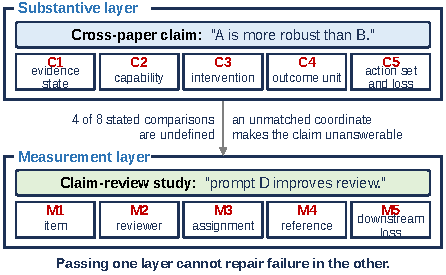
\includegraphics[width=\columnwidth]{figures/generated/fig_two_layer.pdf}%
\caption{The two layers answer different questions about the same sentence.
The substantive layer asks whether two published results concern one decision
problem; Table~\ref{tab:cross-paper-cases} applies it to real comparisons and
supplies the four-of-eight count. The measurement layer asks what a study of
claim review estimates; Table~\ref{tab:retrospective-remedies} shows which
analyses of such a study are valid. Passing one layer cannot repair failure in
the other.}
\label{fig:two-layer}
\end{figure}

\begin{table*}[t]
\centering
\footnotesize
\renewcommand{\arraystretch}{0.92}
\begin{tabularx}{\linewidth}{>{\raggedright\arraybackslash}p{0.18\linewidth}>{\raggedright\arraybackslash}p{0.22\linewidth}>{\raggedright\arraybackslash}p{0.25\linewidth}X}
\toprule
\textbf{Adjacent line} & \textbf{Primary unit} &
\textbf{Unresolved comparison question} & \textbf{This paper's increment} \\
\midrule
General RAG surveys \citep{ragSurvey2024,ragComprehensive2025} &
Architectures, modules, applications &
Whether similarly named gains concern the same evidence state, outcome, and
experimental game &
Adds a claim-level comparison lens and an estimand audit; does not claim a
venue-complete census. \\
Evaluation surveys and unified comparisons
\citep{ragEvaluationSurvey2024,ragBestPractices2024,
alushiRAGComparison2026} &
Metrics, benchmarks, and common-harness reruns &
Which controls are required by a specific cross-study or mechanistic
inference when rerunning is impossible &
Separates scientific coordinates from assignment, participant, item, and
reference units; the simulation quantifies one resulting failure mode. \\
Trustworthy and security RAG surveys
\citep{trustRAGCompass2024,trustworthyRAGSurvey2025,securityRAGSurvey2026} &
Trust dimensions, attack surfaces, and defenses &
Whether benign conflict and attacker-created corruption share a transferable
capability envelope &
Makes origin/access/budget explicit and shows why a prompt-overlapping
reference cannot establish independent criterion validity. \\
Conflict and abstention surveys
\citep{xuKnowledgeConflicts2024,wenAbstentionSurvey2025} &
Conflict types and refusal behavior &
Whether a confidence or sufficiency signal identifies the action that
maximizes utility at a matched operating point &
Separates signal, action, and utility and releases a consequence-defined
counterfactual target without claiming an evaluated policy. \\
\bottomrule
\end{tabularx}
\caption{Positioning relative to adjacent surveys and empirical comparison
work. Each adjacent line partitions the literature by mechanism, which is what a
reader needs to \emph{find} related work. None partitions the
\emph{comparison}, which is what a reader needs when two numbers appear
together, and none is accompanied by evidence that its categories can be read
off a paper. The increment is a reporting-coordinate reduction that is tested
(\S\ref{sec:tested}) and applied at scale (\S\ref{sec:applied}); it is not a
venue-complete systematic review, and it does not supersede these surveys for
discovery.}
\label{tab:main-prior-work-comparison}
\end{table*}

\begin{table*}[t]
\centering
\small
\renewcommand{\arraystretch}{0.92}
\begin{tabularx}{\linewidth}{>{\raggedright\arraybackslash}p{0.13\linewidth}>{\raggedright\arraybackslash}p{0.25\linewidth}>{\raggedright\arraybackslash}p{0.30\linewidth}X}
\toprule
\textbf{Field} & \textbf{Question} & \textbf{Representative values} & \textbf{Why it changes a comparison} \\
\midrule
Evidence state & What is observable at the decision boundary? & Supported; distracting; insufficient; conflicting; stale/weak provenance; adversarially manipulated; not evidence-conditioned. & Query ambiguity and model uncertainty are not silently mixed with properties of retrieved evidence. \\
Origin / capability & How did that state arise, and what can an attacker observe or change? & Benign retrieval; constructed stressor; natural drift/conflict; distribution shift; attacker-created evidence with access, budget, and target. & Transfer depends on the data-generating process and the attacker's capability envelope. \\
Intervention & What part of the system changes? & Corpus/index; retriever; reranker; context assembly; generator; verifier; system control; evaluation artifact. & Components may be alternatives in a shared harness or complementary stages in a pipeline. \\
Outcome & What object and unit are measured? & Answer correctness; retrieval quality; claim support; attack success; privacy leakage; calibration; selective risk; cost. & Identically named datasets do not make different target quantities interchangeable. \\
\textbf{Policy / utility} & What response is selected, under which costs and stakes? & Answer; verify; re-retrieve; expose conflict; clarify; quarantine; recover; abstain; coverage--risk utility. & A signal becomes operational only through an action set and a declared utility context. \\
\midrule
Control check & Does the experiment support the intended inference? & Dataset and corpus snapshot; retriever; top-$k$; generator; decoding; budget; baselines; uncertainty. & Tuple compatibility alone cannot remove experimental confounding. \\
\bottomrule
\end{tabularx}
\caption{The diagnostic schema. The five fields identify whether two results address a compatible question; a claim-specific control check then determines whether their reported numbers support the intended inference. The fields are not assumed orthogonal or sufficient.}
\label{tab:main-framework-overview}
\end{table*}

\begin{table*}[t]
\centering
\scriptsize
\renewcommand{\arraystretch}{0.88}
\begin{tabularx}{\linewidth}{>{\raggedright\arraybackslash}p{0.13\linewidth}>{\raggedright\arraybackslash}p{0.26\linewidth}>{\raggedright\arraybackslash}p{0.30\linewidth}X}
\toprule
\textbf{Coordinate} & \textbf{Controlled values} & \textbf{Equivalence / boundary rule} & \textbf{Verdict effect} \\
\midrule
Evidence state & Supported; irrelevant/distracting; insufficient; conflicting; stale/weak provenance; adversarially manipulated; not evidence-conditioned. & Code what is observable at the decision boundary. Query ambiguity, OOD input, confidence, and attacker access are not evidence states by themselves. & A direct performance claim normally requires a common state or an explicit cross-state estimand. \\
Origin / capability & Benign retrieval; constructed stressor; natural conflict/drift; query or distribution shift; attacker-created evidence; shared clean harness. & Record how the state arose. For security, include corpus write access, query control, retriever visibility, generator access, insertion budget, objective, and target. & A cross-source rank over two different games narrows at best and is otherwise undefined; a shared harness may deliberately vary capability as the controlled factor. \\
Intervention point & Corpus/index; retriever; reranker; context assembly/compression; generator prompting or training; verifier; system-control policy; evaluation-only artifact. & Code the component changed. Different interventions may be compared as alternatives when a shared end-to-end harness controls the remaining pipeline; otherwise they provide component-specific or compositional evidence. & C3 never enters the decision rule. Comparing two different systems means the intervention differs, so a C3 mismatch is the normal state of a comparison and cannot by itself make one undefined; it is recorded so a reader knows what changed. \\
Outcome / unit & Answer correctness; retrieval quality; evidence support; attack or defense utility; privacy leakage; calibration; selective risk/coverage; cost/latency; human preference. & Record definition, direction, aggregation, and unit. Relative gains over different baselines are not automatically a shared estimand. & A one-scalar ranking requires a common target. Without one there is no operating point to re-read at, so the gap is undefined rather than narrowed. \\
Policy / utility & Answer; abstain; re-retrieve; filter; verify; expose conflict; clarify; quarantine; recover; not applicable; unreported. & Use \emph{not applicable} for fixed descriptive comparisons. When policies compete, report action set, stakes, preferences, coverage, and cost. & Different actions can be ranked only under common utility; a signal alone does not establish the preferred response. A stated price at the other side's setting narrows the comparison. \\
Second-stage controls & Dataset/corpus snapshot; retriever/top-$k$/chunking; generator/decoding; compute budget; baselines; uncertainty/statistical design. & Select controls according to the stated inference. The tuple cannot remove confounding from unmatched experimental systems. & Tuple compatibility is necessary diagnostic information but not sufficient for a direct empirical ranking. \\
Final verdict & Survives; narrows; undefined. & Exactly the rule of \S\ref{sec:estimands}, and the only verdict vocabulary used anywhere in this paper or its artifacts. \emph{Survives}: C1, C2, C4 and C5 all match, so the quoted gap stands. \emph{Narrows}: a threatening coordinate differs but a side reports an operating point at the other's setting, or the comparison holds on a strict subset; report that matched number. \emph{Undefined}: no such operating point exists, or a decision-critical field is unavailable after full-text inspection. & Verdicts attach to comparison claims, not permanently to paper pairs, and a new shared-harness experiment can change the supported verdict. An undefined comparison is never replaced by a substitute number computed across the unmatched coordinate. \\
\bottomrule
\end{tabularx}
\caption{The decision procedure of \S\ref{sec:estimands} in full. The five coordinates diagnose semantic compatibility and claim-specific controls determine whether the claim as written is warranted, but only C1, C2, C4 and C5 enter the verdict: C3 is the thing being compared and is recorded rather than tested. The three verdicts here are the same three used in the body, the census codebook and every released artifact.}
\label{tab:framework-decision-procedure}
\end{table*}

\begin{table*}[t]
\centering
\scriptsize
\renewcommand{\arraystretch}{0.9}
\begin{tabularx}{\linewidth}{>{\raggedright\arraybackslash}p{0.20\linewidth}>{\raggedright\arraybackslash}p{0.24\linewidth}>{\raggedright\arraybackslash}p{0.24\linewidth}X}
\toprule
\textbf{Boundary case} & \textbf{Five-coordinate diagnosis} & \textbf{Second-stage control check} & \textbf{Supported conclusion} \\
\midrule
Different interventions, shared harness & A retriever filter and a generator-side reader address the same evidence state, metric target, and answer policy; intervention differs. & Same corpus, retriever output before intervention, generator, budget, metric, and seeds. & A valid end-to-end comparison is possible. Intervention mismatch alone does not force \emph{partial}. \\
All five fields match, systems differ & Two answer-only methods target benign retrieval noise and answer correctness at the generator. & Different datasets, retrievers, model scales, top-$k$, and compute budgets. & The papers are conceptually comparable but their reported numbers are not directly rankable without a shared rerun or adjustment. \\
Action unnamed but observable & A QA benchmark never uses ``action policy'' but requires one answer for every item and gives no abstention channel. & Evaluation code and output schema confirm answer-only behavior. & Code \emph{answer} when policy is decision-relevant; use \emph{not applicable} for a fixed descriptive comparison. \\
Same pair, different claim & An attack artifact and a defense share a threat model but optimise attack success and defended utility. & A common attack--defense harness can evaluate both roles; a paper-only scalar comparison cannot. & Valid as components of one evaluation, partial as substitutable methods, invalid if ranked under incompatible objectives. \\
Same label, incompatible capability & Two poisoning studies both report attack success, but one assumes bounded corpus insertion and the other controls retrieved instructions at query time. & Capability, budget, retrieval probability, and objective do not align. & A direct ranking is invalid even if intervention, metric name, and answer behavior appear similar. \\
\bottomrule
\end{tabularx}
\caption{Counterexamples delimiting the schema. Verdicts depend on the stated comparison and experimental controls; the five coordinates are diagnostic fields rather than a necessary-and-sufficient classifier.}
\label{tab:framework-counterexamples}
\end{table*}

\begin{table*}[t]
\centering
\scriptsize
\renewcommand{\arraystretch}{0.88}
\begin{tabularx}{\linewidth}{>{\raggedright\arraybackslash}p{0.18\linewidth}c c c c >{\raggedright\arraybackslash}p{0.15\linewidth}X}
\toprule
\textbf{Threat class} & \textbf{Corpus} & \textbf{Query} & \textbf{Retr.} & \textbf{Gen.} & \textbf{Objective} & \textbf{Boundary} \\
\midrule
Dense-retriever poisoning \citep{poisoningRetrievalCorpora2023} & write & train set & white/gray & no & retrieve bad passages & Not always end-to-end. \\
RAG knowledge corruption \citep{poisonedRAG2024,badRAG2024} & write & target topic & black/gray & black & answer steering & Stealth/dynamics vary. \\
Backdoor-style RAG \citep{trojanRAG2024,phantom2024} & write & trigger & gray & black & latent behavior & Normal queries may pass. \\
Indirect prompt injection \citep{aip2025,rrag005} & write/share & natural & black & black & instruction hijack & Must overcome retrieval. \\
Opinion/fairness manipulation \citep{rrag104,rrag162} & write & group/topic & black/gray & black & bias steering & QA metrics miss social harm. \\
Defense setting \citep{certifiedRAG2024,rrag004,rrag015,rrag128} & bounded & varies & assumed & black/gray & detect/demote/trace & Depends on budget/visibility. \\
\bottomrule
\end{tabularx}
\caption{Attacker-capability matrix for adversarial RAG. The same ``attack success rate'' can mean different things depending on corpus write access, query control, retriever visibility, generator access, and objective.}
\label{tab:attacker-capability}
\end{table*}


\FloatBarrier
\section{Evaluation and Reporting}
\label{sec:appendix-eval}
\begin{table*}[t]
\centering
\scriptsize
\renewcommand{\arraystretch}{0.9}
\begin{tabularx}{\linewidth}{>{\raggedright\arraybackslash}p{0.18\linewidth}>{\raggedright\arraybackslash}p{0.30\linewidth}>{\raggedright\arraybackslash}p{0.22\linewidth}X}
\toprule
\textbf{Required field} & \textbf{What to report} & \textbf{If omitted} & \textbf{Example consequence} \\
\midrule
Evidence-state definition & Supported, irrelevant/distracting, insufficient, conflicting, stale/weak provenance, adversarially manipulated, or not evidence-conditioned. & Papers with the same robustness label may test different evidence properties. & Noise training is ranked against sufficiency prediction. \\
Origin / capability & Benign retrieval, constructed stressor, natural conflict/drift, distribution shift, or attacker access, budget, objective, and target. & Stressors are not portable. & Natural conflict is compared with poisoning. \\
Intervention boundary & Corpus/KB, retriever/context, context assembly, generator, system control, or evaluation artifact. & Pipeline modules are treated as substitutable. & A benchmark is ranked against a mitigation method. \\
Retrieval setting & Corpus snapshot, retriever, top-$k$, chunking, reranking/compression, and index drift controls. & Results cannot be reproduced or normalised. & A filter looks better because its retriever retrieved easier negatives. \\
Outcome and unit & Answer correctness, support, attack success, privacy leakage, selective risk, calibration, cost, or action utility, including definition and aggregation. & Different objectives collapse into one score. & Lower attack success hides clean-utility loss. \\
Policy and utility & Answer, abstain, retrieve again, filter, verify, expose conflict, clarify, quarantine, or recover, plus stakes, preferences, coverage, and cost when actions compete. & Accuracy and confidence are over-interpreted. & A calibrated answerer may still answer from insufficient evidence. \\
Model and comparison controls & Dataset, generator, decoding, compute budget, baselines, seeds, uncertainty intervals, and significance procedure. & Tuple-aligned papers can still be empirically confounded. & A method appears better because it uses a stronger generator or a larger budget. \\
Uncertainty / abstention handling & Coverage, selective risk, confidence target, abstention reward, and re-retrieval cost. & Abstention can hide retrieval failure. & Refusal is rewarded when re-retrieval should be the correct action. \\
Security threat model & Attacker access, query control, retriever visibility, insertion budget, objective, and adaptive-defense assumptions. & Security numbers are not comparable. & Prompt injection defenses are claimed to protect against corpus poisoning. \\
\midrule
Provenance of every quoted number & Whether the other side's figure was \emph{transported} from its paper or \emph{re-implemented} in this harness, and at which configuration. & The one property an automated audit recovers reliably ($\kappa$ \DecProvK{}) is lost, and the stratum where incomparability lives cannot be found. & A re-implementation at a strengthened attack budget reads as a defeat of the published attack. \\
Reviewer/judge panel and unit map & Who or what adjudicated, how many, which items each saw, and how any prompt or instruction was assigned across them. & The unit of assignment is unrecoverable, so uncertainty cannot be computed at the unit that was varied. & A source-level test rejects a true null $\SimAtCensus\%$ of the time at the heterogeneity measured here. \\
Pre-aggregation votes & Per-reviewer labels with stable reviewer identifiers, before adjudication or majority voting. & Only reviewer-level analyses hold their nominal size, and they need these votes. & A reported agreement rate cannot be converted into a valid reviewer-level test after the fact. \\
\bottomrule
\end{tabularx}
\caption{Reporting checklist for robust RAG under unreliable evidence, in the order of \S\ref{sec:practice}. The first block is the five coordinates and the controls that accompany them. \S\ref{sec:instrument} shows why they head the list: a comparison whose answer turns on a coordinate the paper does not state is the one case in which a panel neither agrees nor is right, and C1 and C4 are the two fields whose absence produces that case most often. The last block is what the audit of the audit requires.}
\label{tab:robust-rag-reporting-checklist}
\end{table*}

\begin{table*}[t]
\centering
\scriptsize
\renewcommand{\arraystretch}{0.95}
\begin{tabularx}{\linewidth}{>{\raggedright\arraybackslash}p{0.12\linewidth}>{\raggedright\arraybackslash}p{0.13\linewidth}>{\raggedright\arraybackslash}p{0.17\linewidth}>{\raggedright\arraybackslash}p{0.18\linewidth}>{\raggedright\arraybackslash}p{0.14\linewidth}X}
\toprule
\textbf{Benchmark} & \textbf{Risk focus} & \textbf{Task / data} & \textbf{Perturbation or threat} & \textbf{Metrics} & \textbf{Boundary} \\
\midrule
RGB \citep{rgb2023} & noise, rejection, integration, counterfactuality & English/Chinese QA & noisy passages, false evidence, negative evidence & accuracy, ability-specific scores & Broad diagnostic benchmark but not adaptive attack-oriented. \\
RAGTruth \citep{ragTruth2024} & hallucination / faithfulness & QA, data-to-text, summarization & naturally generated unsupported spans & word-level hallucination labels & Strong annotation granularity; less focused on retrieval-side threat models. \\
Sufficient Context \citep{sufficientContext2024} & answerability & QA with context sufficiency labels & insufficient retrieved evidence & selective generation / abstention & Captures answerability but not adversarial corruption. \\
MagicMushroom \citep{rrag027} & retrieval noise & configurable RAG stress tests & distracting, low-quality, inconsequential, irrelevant noise & robustness under noise types & Fine-grained noise; limited conflict/security coverage. \\
URAG \citep{rrag001} & uncertainty & RAG as MCQA / conformal prediction & irrelevant/noisy retrieval and uncertainty sets & coverage, set size, calibration & Good for uncertainty; less direct for free-form generation. \\
QueryRobust \citep{queryRobustness2025} & query robustness & QA with query perturbations & wording variation at query--retrieval interface & retrieval and end-task degradation & Focuses on query perturbation, not corpus corruption. \\
PoisonArena \citep{rrag023} & adversarial poisoning & RAG attack competition setting & competing poisoning attacks & attack success, retrieval effects & Strong security focus; benign uncertainty is secondary. \\
SafeRAG \citep{rrag019} & RAG security & security benchmark for RAG & poisoning / malicious retrieval contexts & attack and defense metrics & Security-oriented; not a full evidence reliability suite. \\
MTRAG-UN \citep{rrag141} & multi-turn unanswerability & multi-turn RAG conversations & unanswerable, underspecified, non-standalone questions & abstention / clarification quality & Covers interaction; less focused on adversarial evidence. \\
CRUMQs \citep{rrag193} & unanswerable multi-hop RAG & realistic multi-hop queries & unanswerable and uncheatable questions & answerability and robustness & Useful for abstention; not a broad attack/noise benchmark. \\
\bottomrule
\end{tabularx}
\caption{Benchmark-level comparison for robust RAG evaluation. The table makes explicit what each benchmark perturbs, what it measures, and which failure modes remain outside its scope.}
\label{tab:benchmark-comparison}
\end{table*}


\begin{table*}[t]
\centering
\scriptsize
\renewcommand{\arraystretch}{0.9}
\begin{tabularx}{\linewidth}{>{\raggedright\arraybackslash}p{0.24\linewidth}>{\raggedright\arraybackslash}p{0.25\linewidth}>{\raggedright\arraybackslash}p{0.21\linewidth}X}
\toprule
\textbf{Main claim} & \textbf{Cited evidence basis} & \textbf{What the evidence supports} & \textbf{Boundary} \\
\midrule
Irrelevant or noisy context can harm generation. & Irrelevant-context robustness, RAAT, RGB, and counterfactual-noise studies. & Noise affects both retrieval quality and generator context use. & Does not imply one robustness score covers all noise types. \\
Knowledge conflict differs from adversarial corruption. & Conflict and poisoning studies with different evidence origins and evaluation targets. & Natural disagreement and attacker-created contradiction require different assumptions. & Conflict-resolution results should not be read as poisoning-defense results. \\
RAG attacks require capability normalisation. & Poisoning, backdoor, prompt-injection, traceback, and certification studies. & Attack/defense results require corpus access, query control, retriever visibility, and budget. & The paper does not rank attacks by real-world prevalence. \\
Calibration, abstention, and retrieval control are distinct. & Sufficient-context, uncertainty, adaptive-retrieval, and calibration studies. & Confidence estimation, evidence sufficiency, retrieval triggering, and abstention optimise different quantities. & Does not validate a single universal control policy. \\
Action-trace evaluation is a benchmark agenda. & Benchmarks exposing subsets of answer, evidence, action, cost, and threat fields. & Existing benchmarks cover pieces of the proposed schema. & No new leaderboard or empirical system ranking is claimed. \\
\bottomrule
\end{tabularx}
\caption{Narrative claim-to-source ledger. Expanded and strict citation audits
were model-assisted and deterministic; this table records the intended evidence
boundary rather than certifying every citation.}
\label{tab:claim-verification-ledger}
\end{table*}


\FloatBarrier
\section{Scoping-Map Audit Artifacts}
\label{sec:audit-artifacts}
\begin{table*}[t]
\centering
\small
\renewcommand{\arraystretch}{0.95}
\begin{tabularx}{\linewidth}{>{\raggedright\arraybackslash}p{0.16\linewidth}>{\raggedright\arraybackslash}p{0.19\linewidth}>{\raggedright\arraybackslash}p{0.25\linewidth}>{\raggedright\arraybackslash}X}
\toprule
\textbf{Evidence layer} & \textbf{Unit and size} & \textbf{Structured coverage} & \textbf{Supported use and provenance boundary} \\
\midrule
Scoping corpus & 536 broadly included papers & Metadata and broad relevance & Documentary recall pool; single model-assisted broad screen, not duplicated and not prevalence-estimating. \\
Map B & 342 paper rows & Literature family and intervention; free-text metrics; no structured evidence origin or policy & Source-stratified landscape synthesis; adjudicated subsets, but not a five-coordinate map. \\
Claim inventory & 289 claims from purposive fixed sections & Model-coded coordinates, evidence flags, and claim-specific controls & Source-linked hypothesis index; its verdict distribution and internal ablations are not validated results. \\
Instrument benchmark & 360 constructed comparability items & Five coordinate values and a verdict fixed when each item is written; six judges from three developers under three codebooks & The instrument claim of \S\ref{sec:instrument}. Templated prose, so it bounds what the schema can do on text that states it, not on any particular published passage. \\
Cross-paper census & 1,703 frame windows & Nine judges, fully crossed, one codebook & The prevalence and reliability claims of \S\ref{sec:census}. No verdict-based rate is an estimate. \\
\bottomrule
\end{tabularx}
\caption{The released evidence layers answer different questions. Larger
model-assisted layers do not validate claim-level verdicts; the human layers
test an annotation procedure rather than literature prevalence. No layer is
treated as an independently validated gold standard.}
\label{tab:main-evidence-layers}
\end{table*}

% Drawn by scripts/revision3/fig_appendix_flows.py; the .pptx is the editable
% source and is released with the paper.
\begin{figure*}[t]
\centering
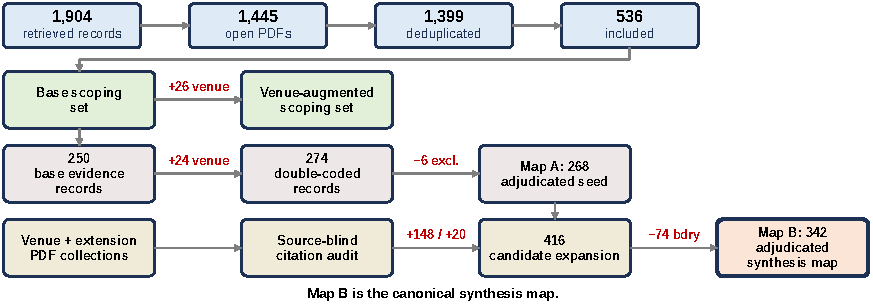
\includegraphics[width=\textwidth]{figures/generated/fig_corpus_lineage.pdf}%
\caption{Corpus lineage. Red deltas on the connectors are, in order, $+26$ and
$+24$ venue-linked additions, $-6$ exclusions, $+148$ new and $+20$ enriched
rows from the citation audit, and $-74$ boundary rows removed at adjudication.
The 416-row venue-expanded candidate map is second-coded and adjudicated into
Map~B (342 rows), the canonical synthesis evidence map. Map~A (268 rows) is the
double-coded adjudicated seed used for IAA and adjudication audit; the base and
venue-augmented scoping sets are used only for boundary checks, while a separate
300-paper source-blind citation audit over the venue and extension PDF
collections decides which papers enter the main text, case studies, or
appendix.}
\label{fig:corpus-flow}
\end{figure*}

\begin{table*}[t]
\centering
\small
\begin{tabularx}{\linewidth}{p{0.18\linewidth}p{0.16\linewidth}X}
\toprule
\textbf{Stage} & \textbf{Count} & \textbf{Rule} \\
\midrule
Initial retrieval & 1,904 records & Keyword search over arXiv, ACL Anthology, OpenReview, USENIX, AAAI/ACM landing pages where open versions were available, plus curated robust/trustworthy RAG paper lists; search cutoff 2026-06-03. \\
Open full-text corpus & 1,445 PDFs & Downloaded only open PDFs; removed failed downloads, inaccessible files, and non-PDF artifacts. \\
Deduplicated candidates & 1,399 papers & Deduplicated by normalised title and arXiv/proceedings identifiers; retained the most complete metadata record when preprint and proceedings versions overlapped. \\
Relevance screening & 536 included papers & Included papers that study RAG robustness, reliability, uncertainty, calibration, faithfulness, attack/defense, or evaluation under unreliable evidence; excluded application-only RAG papers. \\
Core pool & 112 papers & Papers directly shaping the taxonomy, threat/failure model, intervention mechanisms, or evaluation framework. \\
Core reading set & 100 papers & Core papers used as main narrative anchors; the remaining 12 core-pool papers stay in the broader scoping set. \\
Base scoping set & 300 papers & Core papers plus representative supporting work across all taxonomy branches before venue follow-up triage. \\
Venue-augmented scoping set & 326 papers & Base scoping set plus 26 venue-linked additions after follow-up triage. \\
Candidate evidence records & 274 papers & Base evidence map of 250 papers plus 24 venue-linked additions, double-coded and adjudicated. \\
Map A adjudicated seed & 268 papers & Candidate evidence records retained after final adjudication; used for IAA/adjudication provenance. \\
Map-B candidate expansion & 416 papers & Map A plus 148 source-blind human-citation-audit additions and 20 enriched original rows; used for second-coding review. \\
Map B adjudicated synthesis map & 342 papers & Map A plus 74 retained additions after second coding and final adjudication; frozen for current descriptive statistics. Post-freeze discoveries enter a recall log until a new version is coded. \\
\bottomrule
\end{tabularx}
\caption{Screening-flow summary. Search ends on 2026-06-03; coding and adjudication artifacts freeze on 2026-06-15. The supplement provides query strings, source counts, rules, exclusions, hashes, and a post-freeze recall log.}
\label{tab:review-protocol}
\end{table*}

\begin{table*}[t]
\centering
\scriptsize
\renewcommand{\arraystretch}{0.92}
\begin{tabularx}{\linewidth}{>{\raggedright\arraybackslash}p{0.20\linewidth}>{\raggedright\arraybackslash}p{0.15\linewidth}>{\raggedright\arraybackslash}p{0.30\linewidth}X}
\toprule
\textbf{Artifact / set} & \textbf{Count} & \textbf{Count definition} & \textbf{Use in this paper} \\
\midrule
Map-A double-coded candidates & 274 & Candidate records coded by two human sources before final inclusion adjudication. & Used for human-human agreement and adjudication; six records were excluded from Map A. \\
Map A adjudicated seed & 268 & Included records after adjudication: 42 venue/proceedings-linked, 222 arXiv-only or emerging preprints, 2 preprints with year tags, 1 review-platform record, and 1 other/uncategorized record. & Used as the IAA/adjudication provenance snapshot, not the current synthesis denominator. \\
Venue-augmented scoping set & 326 & Original base scoping set plus 26 triaged venue-linked additions. & Used for broader scoping and boundary checks; not all rows are evidence-map records. \\
Source-blind citation audit & 300 & Human citation decisions over venue PDFs and extension PDFs. & Determines which audited papers enter the main text, case studies, appendix, background, or exclusion set; distinct from the base scoping set. \\
Map-B candidate expansion & 416 & Map A plus 148 candidate additions supported by the source-blind citation audit; 20 original rows enriched with citation-audit metadata. & Pre-adjudication expansion candidate map used for second-coding review. \\
Map B adjudicated synthesis map & 342 & Map A plus 74 retained additions after second coding and final adjudication. & Current evidence map for source-stratified synthesis and Map-B cross-tabs. \\
\bottomrule
\end{tabularx}
\caption{Reconciliation of reported corpus counts. The 342-row adjudicated Map B is the canonical synthesis map; Map A and the 274-candidate set are retained to report double-coding and adjudication provenance.}
\label{tab:source-strata-reconciliation}
\end{table*}


\FloatBarrier
\end{document}
